%
% skript.tex -- Lecture notes for the PartDiff lectures given at the
%               MSE Master
%
% (c) 2006-2018 Prof. Dr. Andreas Mueller, HSR
%
\documentclass[a4paper,12pt]{book}
\usepackage[utf8]{inputenc}
\usepackage[T1]{fontenc}
%\usepackage{german}
\usepackage{times}
\usepackage{geometry}
\usepackage{csquotes}
\geometry{papersize={210mm,297mm},total={160mm,240mm},top=31mm,bindingoffset=15mm}
\usepackage{amsmath}
\usepackage{amssymb}
\usepackage{amsfonts}
\usepackage{amsthm}
\usepackage{amscd}
\usepackage{graphicx}
\usepackage{fancyhdr}
\usepackage{textcomp}
\usepackage{txfonts}
\usepackage[all]{xy}
\usepackage{paralist}
%\usepackage[colorlinks=true]{hyperref}
\usepackage{hyperref}
\usepackage{array}
\usepackage{tikz}
\usepackage{pdfpages}

%für Querformat von zeitplan
\usepackage{pdflscape}

%für Abbreviations
\usepackage{acronym}

%figure float
\usepackage{float}

%für python code
\usepackage{listings}

%bibliography
\usepackage[hyperref=true,backend=biber,style=ieee,defernumbers=true]{biblatex}
\addbibresource{references.bib}

%%%%%%%%%%%%%%%%%%%%%%%
%% Copyleft
%% Walter A. Kehowski
%% Department of Mathematics
%% Glendale Community College
%% walter.kehowski@gcmail.maricopa.edu
%% \begin{linsys}{2}
%% -x & + & 4y & = & 8\\
%% -3x & - & 2y & = & 6
%% \end{linsys}
%%%%%%%%%%%%%%%%%%%%%%%
%\makeatletter
%% math-mode column types ------------------
\newcolumntype{\linsysR}{>{$}r<{$}}
\newcolumntype{\linsysL}{>{$}l<{$}}
\newcolumntype{\linsysC}{>{$}c<{$}}
\newenvironment{linsys}[1]{%
\begin{tabular}{*{#1}{\linsysR@{\;}\linsysC}@{\;}\linsysR}}%
{\end{tabular}}
%\makeatother
\endinput

\makeindex


\begin{document}
\pagestyle{fancy}
\lhead{}
\rhead{}
\frontmatter
\newcommand\HRule{\noindent\rule{\linewidth}{1.5pt}}



\hypersetup{
	colorlinks=true,
	linktoc=all,
	linkcolor=blue
}


\newtheorem{satz}{Theorem}[chapter]
\newtheorem{problem}[satz]{Problem}
\newtheorem{hilfssatz}[satz]{Lemma}
\newtheorem{definition}[satz]{Definition}
\newtheorem{annahme}[satz]{Assumption}
\newtheorem{aufgabe}[satz]{Task}
\newenvironment{beispiel}[1][Example]{%
	\begin{proof}[#1]%
		\renewcommand{\qedsymbol}{$\bigcirc$}
	}{\end{proof}}
%\allowdisplaybreaks


\begin{titlepage}
\vspace*{\stretch{1}}
\HRule
\vspace*{10pt}
\begin{flushright}
{\Huge
Low-Power Wakeup Receiver}

%\Large{with Rotation, GPS and On-Board-Diagnostics Sensor Data}
\end{flushright}
\begin{flushright}
{\Large Semester Thesis 2019}
\end{flushright}
\HRule

\vspace{70pt}
\large
\textbf{Authors}

Cédric Renda, Manuel Tischhauser

\textbf{Supervisor}

Prof. Dr. Heinz Mathis

\textbf{Assistant Supervisor}

Selina Malacarne

\textbf{Subject}

Wireless Communications



\vspace*{\stretch{2}}
\begin{center}
HSR Hochschule Für Technik Rapperswil

\today
\end{center}
\end{titlepage}


\chapter*{Abstract}

\section*{Introduction}
In company buildings, universities and other similar facilities, it is usual to attach occupancy schedules next to room entrances. These schedules are most of the time printed on paper, or in more modern buildings, displayed on a screen. Using paper, it is impracticable to take short-term changes into account, since every adjustment needs to be made by printing a new schedule. Screens on the other hand need either to be connected to the power grid, which entails extensive installation work, or powered by a battery, which needs to be replaced from time to time. All these disadvantages could be avoided by using a screen which harvests its energy from the indoor light, and is updated via a wireless interface. The screen should therefore be completely wireless.

\section*{Approach}
Energy is harvested with solar cells and is stored in a super-capacitor.
Because this harvesting unit cannot provide unlimited energy, the whole system with display, microcontroller and wireless interface should consume as little energy as possible.
To achieve this, an e-paper display is used, which only needs energy to update the screen, but not to maintain the displayed image.
A constantly listening wakeup receiver can generate an wakeup interrupt and makes a periodic wake up of the microcontroller to check for incoming events redundant while maintaining a reasonable response time.
A lot of energy can be saved this way, since updating the screen usually doesn't happen more than a few times a week.

\section*{Conclusion}
Energy harvesting provides enough energy if updating of the schedule does not occur to frequently. This semester thesis shows, that a wakeup receiver is suitable for this kind of problem. By implementing a self-holding circuit, it is even possible to switch off the whole system (except wakeup receiver) when unused. The wakeup receiver consumes in this listening mode $4.5\,\mu\text{W}$ at most.
\tableofcontents

\mainmatter

\chapter*{Abbreviations}
\addcontentsline{toc}{chapter}{Abbreviations} 

\begin{acronym}
	\acro{fraun}[IIS]{Fraunhofer-Institut für Integrierte Schaltungen}
\end{acronym}

\begin{acronym}
	\acro{ask}[ASK]{Amplitude Shift Keying}
\end{acronym}

\begin{acronym}
	\acro{ook}[OOK]{On-Off Keying}
\end{acronym}

\begin{acronym}
	\acro{gui}[GUI]{Graphical User Interface}
\end{acronym}

\begin{acronym}
	\acro{spi}[SPI]{Serial Peripheral Interface}
\end{acronym}
\chapter{Introduction}
In company buildings, universities and other similar facilities, it is usual to attach occupancy schedules next to room entrances.
These schedules are mostly printed on paper, or in more modern buildings, displayed on a screen.
Using paper, it is impracticable to take short-term changes into account, since every adjustment needs to be made by printing a new schedule.
Screens on the other hand need either to be connected to a power supply, which entails extensive installation work, or are powered by a battery, which needs to be replaced from time to time.
All these disadvantages could be avoided by using a screen which can be updated wireless and is in itself autarkic.
The goal of this semester thesis is to develop a functional prototype of such a schedule.
To keep the energy consumption at a minimum, a low-power wakeup receiver is used.

\section{Task analysis}
The prototype should combine both the advantages of the paper method and the screen.
Updating should happen via a wireless interface while a expensive installation should be avoided.
The screen should therefore be placed on the desired location  just like a paper schedule.
To consume as low power as possible, the microcontroller, display and interface should be switched off when not needed.

\section{Approach}
To simplify the description, from now on the display with all its components is called the receiver, while the other end, a computer with additional hardware is called the transmitter.
This does not mean, that the communication is uni-directional, since both ends should be able receive and transmit data, but more that the general data transfer happens from the computer to the screen.

\paragraph{Transmitter}
This end only consists of a computer, a wireless interface for the main communication and the transmitter module of the wakeup receiver.
A short python script enables the user to define which data the receiver should print over a fixed template.
Information is transferred to a wireless interface which transmits it to the receiver end after the receiver is woken up.

\paragraph{Receiver}
This part of the prototype should consume as low power as possible.
An e-paper display is used, because it is bi-directional, which means it can maintain its image even when disconnected of the power supply.
A wireless module receives information from the transmitter and, if needed, sends back feedback about the status.
This connection should therefore be bi-directional.
To process the incoming data and display it correctly on the screen, a microcontroller is needed.
All these components are completely disconnected from the power supply when not used.
The power is provided by a super capacitor which is charged by solar cells.
When switched off, the only component which actively consumes power is a wakeup receiver.
This module is constantly in listening mode and waits for a wakeup event.
Is such an event received, it activates a self-holding circuit which connects the power supply to the other components.
Data can now be exchanged over a different channel, established by the wireless module.
After the data is processed and the display is refreshed, the microcontroller deactivates the self-holding circuit and disconnects in this step itself and all other components except the wakeup receiver from the power source. 
\chapter{Theory}

\section{E-Paper Display}
There are several different technologies which are applied in e-paper displays.
Since the developed prototype uses a microencapsulated electrophoretic display, this section only describes this specific implementation.

A film consisting of microscopic capsules is coated onto a backplane, which basically is a matrix of electrodes.
On top of that comes a common electrode, called the frontplane.
This setup is shown in Figure \ref{theory:capsules}.

\begin{figure}[ht]
	\centering
	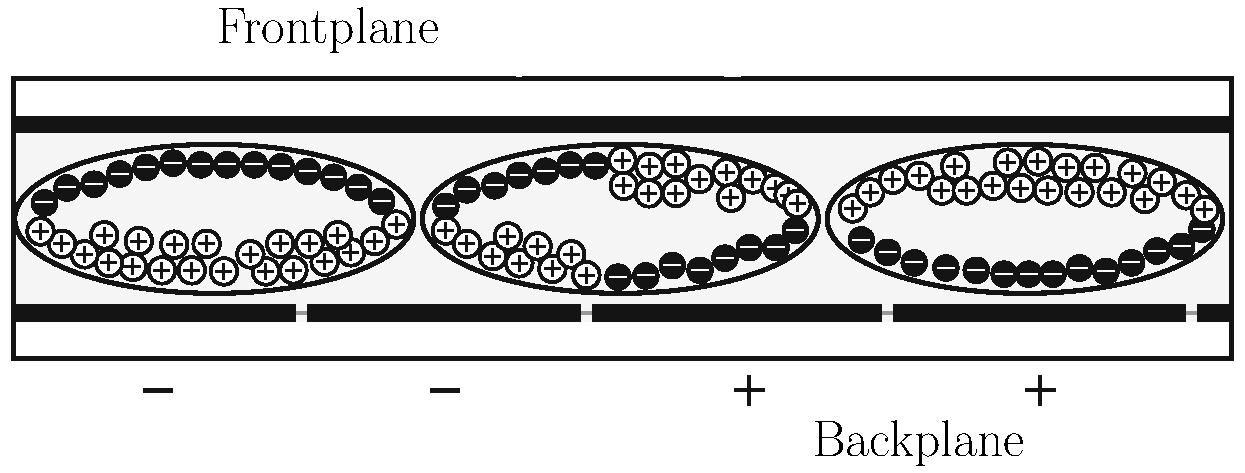
\includegraphics[width=0.9\textwidth]{2-theory/e-paper-display/graphics/capsules.pdf}
	\caption{Capsules between to electrodes (taken from \cite{amundson} with adjustments).\label{theory:capsules}}
\end{figure}

Each capsule in the film itself contains a transparent fluid and particles of two opposite charges.
One type of particle scatters the light while the other one absorbs it.
The particles now begin to move in opposite directions through the fluid when exposed two an electrical field. 
The pixel (defined by the electrode size) appears white if the scattering particles are near the frontplane and black if otherwise.
If no voltage is applied to the electrodes, the particles maintain their last position.
This makes it possible, to switch off the power supply when no image update is needed. 
This is the reason why the power consumption can be strongly reduced compared to other types of display \cite{amundson}.

\begin{figure}[ht]
	\centering
	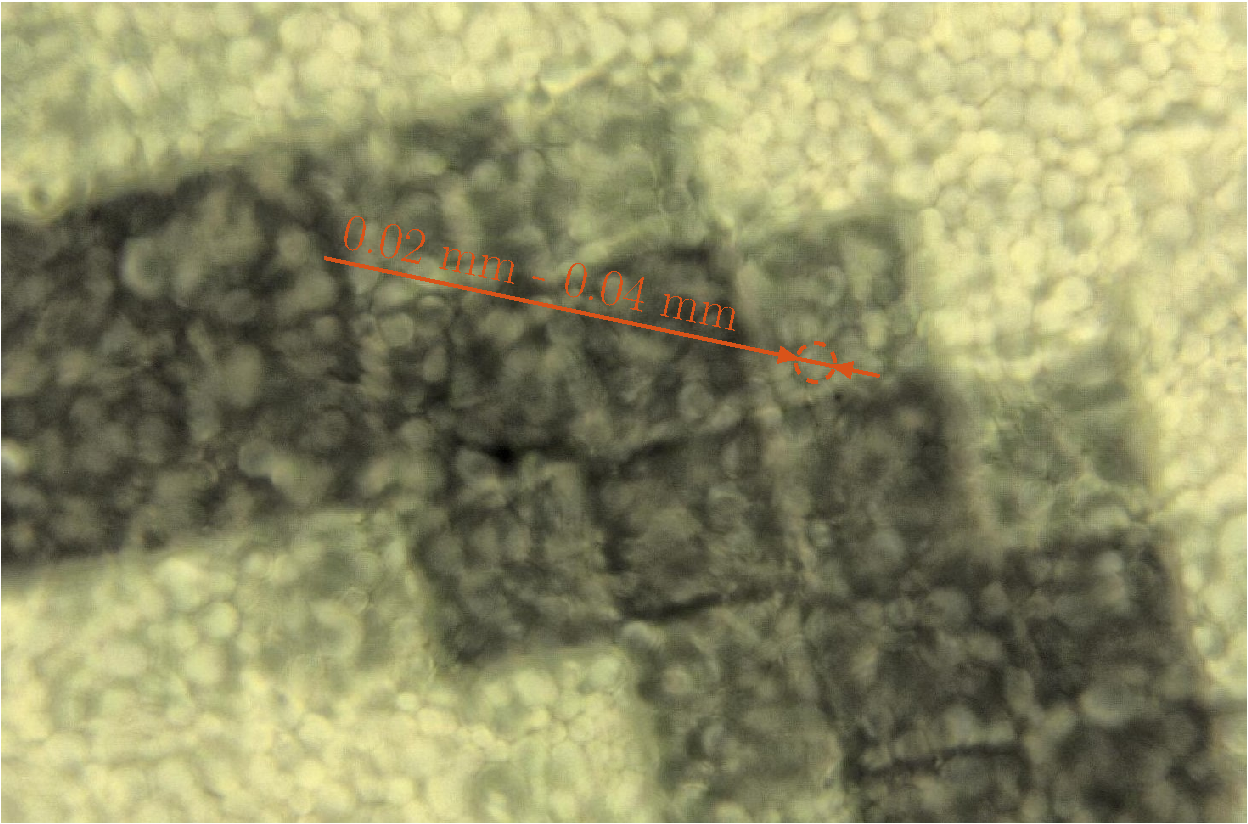
\includegraphics[width=0.9\textwidth]{2-theory/e-paper-display/graphics/epaper_mikroskop.pdf}
	\caption{E-paper display under microscope with 250x magnification.\label{theory:micro}}
\end{figure}

Figure \ref{theory:micro} shows an e-paper display with 250x magnification.

\section{Wakeup Receiver}
In order to reduce power with a conventional receiver it has to be programmed to stay in sleeping mode until it is used again. However, it has to check whether any data was sent, therefore, it has to wake-up periodically to check if any notifications were sent. This duty cycle is a trade-off between power consumption and the respective response time. Conclusively, if the period between the notification checks is longer, the receiver is in an extended sleeping mode using less power, but simultaneously potentially missing out on a new notification, as the data can only be received in the running mode. The wakeup receiver now allows the device to be constantly in the listening mode, while consuming just a small amount of energy. Additionally to the system, the actual microcontroller, which coordinates the data transmission and other tasks stays shut down with only the wakeup receiver in listening mode. After receiving a defined pattern over this channel, the wakeup receiver generates an interrupt resulting in waking up the microcontroller. Subsequently, it establishes now a channel over a different wireless module, or execute another task. When finished, the microcontroller puts itself and all other modules (except the wakeup receiver) in sleep mode again. Figure \ref{theory:wake} shows a comparison of both the conventional approach and the solution with the wakeup receiver.
\begin{figure}[ht]
	\centering
	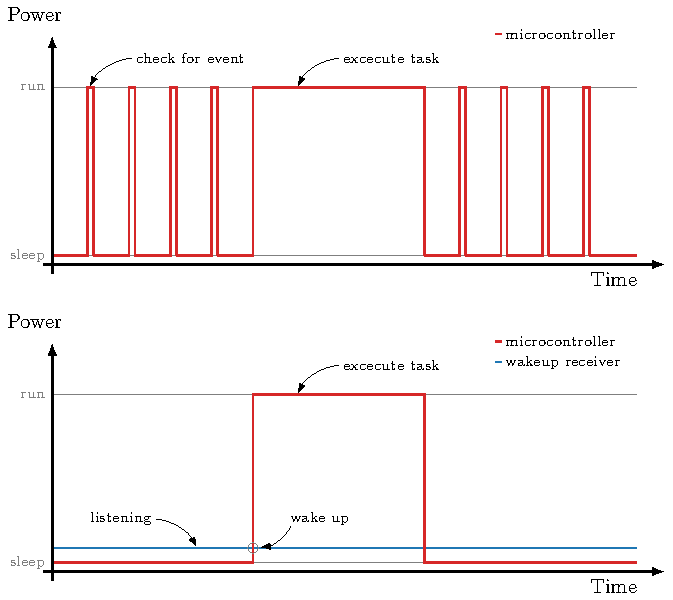
\includegraphics[width=0.9\textwidth]{2-theory/wakeup/graphics/wake_comp.pdf}
	\caption{Top: Microcontroller checks periodically for incoming data. Bottom: Constantly listening  wakeup receiver.\label{theory:wake}}
\end{figure}

One could argue, that the wakeup receiver module consumes in general more power, than the
microcontroller in sleep mode. However, since the microcontroller only wakes up when a task needs to be done, the overall energy consumption (area underneath the curve) is going to be smaller if the occurring wakeup event comes infrequently or over longer periods of time. The response time on the other hand can be kept in the microsecond range.


\section{Drawing graphics on a graphics display}
\label{chapter:DrawGraph}

If a matrix style display is used with a microcontroller, there are a lot of different ways to draw graphical elements. This section covers only the ways used in this project. 

\subsubsection{Matrix displays}
Since most displays produced have a rectangular shape, the amount of pixel they hold is calculated like the surface of an rectangular. The number of pixels on both axis are multiplied and we get the total amount of pixels we have to manipulate. So it is obvious that the memory size of a picture explodes with its resolution. A display with a size of $1200 \times 825$ pixels and a colour depth of 24 bit serves as an example. This resolution results in amount of $1200\cdot825=990'000$ pixels and thus $1200\cdot825\cdot24=23'760'000$ bits. This is a huge amount of data to process with a standard microcontroller.
To handle the data transfer between memory and display, special parallel driver chips are used. These drivers are mapping the right memory location to the desired pixel on the display. More expensive driver chips have built in memory. To access it from a host \acs{cpu}, parallel or serial bus interfaces are used. If a display is rectangular, the information with the pixel value can be ordered in a matrix.
A good option to store an image is therefore an array.
The advantage of an array is the easy access and the memory allocation given in various programming languages.
In C for example, memory of an array has to be allocated at consecutive addresses \cite{ISO/IEC9899}.
 
% \begin{align}
%n = \lfloor \log_{2}(176) \rfloor = 8 bit.
% \end{align}

% bit.   

%\begin{figure}[H]
%	\centering
%	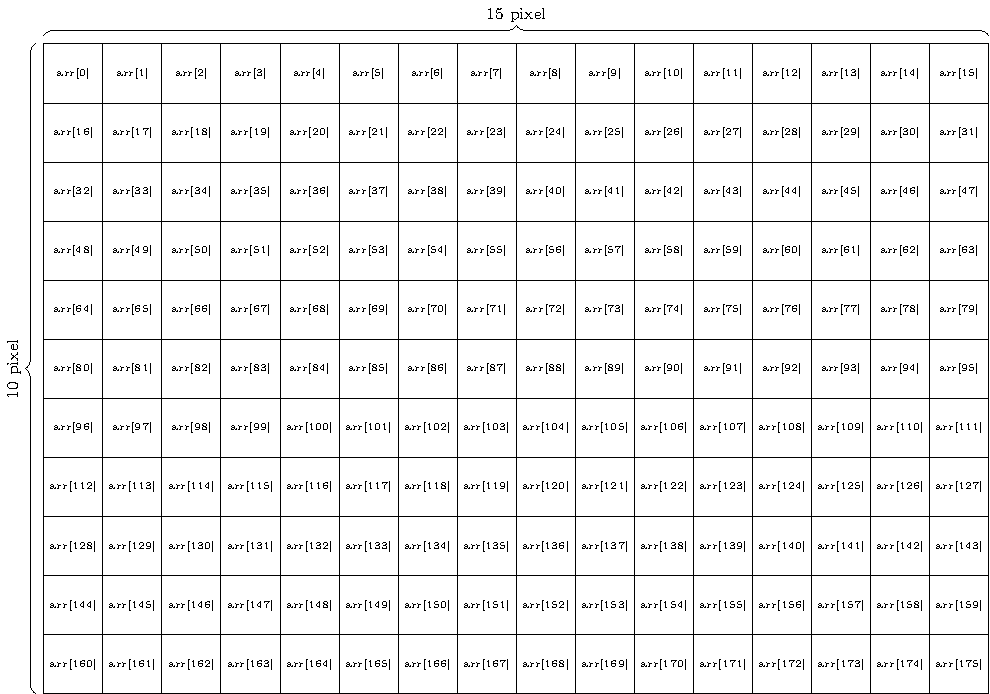
\includegraphics[width=1\textwidth]{2-theory/drawing-graphics/graphics/matrix.pdf}
%	\caption{$16\times 11$ pixel display with a flat matrix \label{theory:matrix}}
%\end{figure}

% \begin{align}
%n = \lfloor \log_{2}(11) \rfloor + \lfloor\rfloor\log_{2}(16) \rfloor = 8 bit.
%\end{align}

%\begin{figure}[H]
%	\centering
%	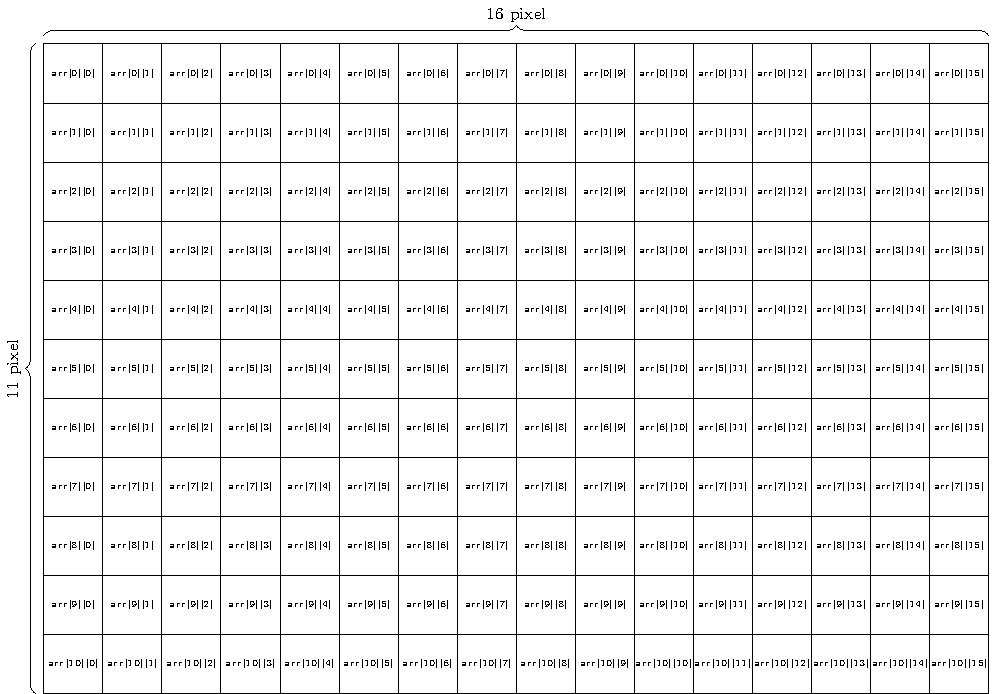
\includegraphics[width=1\textwidth]{2-theory/drawing-graphics/graphics/matrix2.pdf}
%	\caption{$16\times 11$ display with a two dimensional matrix\label{theory:matrix2}}
%\end{figure}

\subsubsection{Double buffering}
To write an image to a display, two separate memory accesses are carried out.
The first writes the image into the buffer, the second takes this data and displays on screen.
By using two buffers, it is possible to accelerate this process.
This is shown in Figure \ref{theory:buffer}.

\begin{figure}[ht]
	\centering
	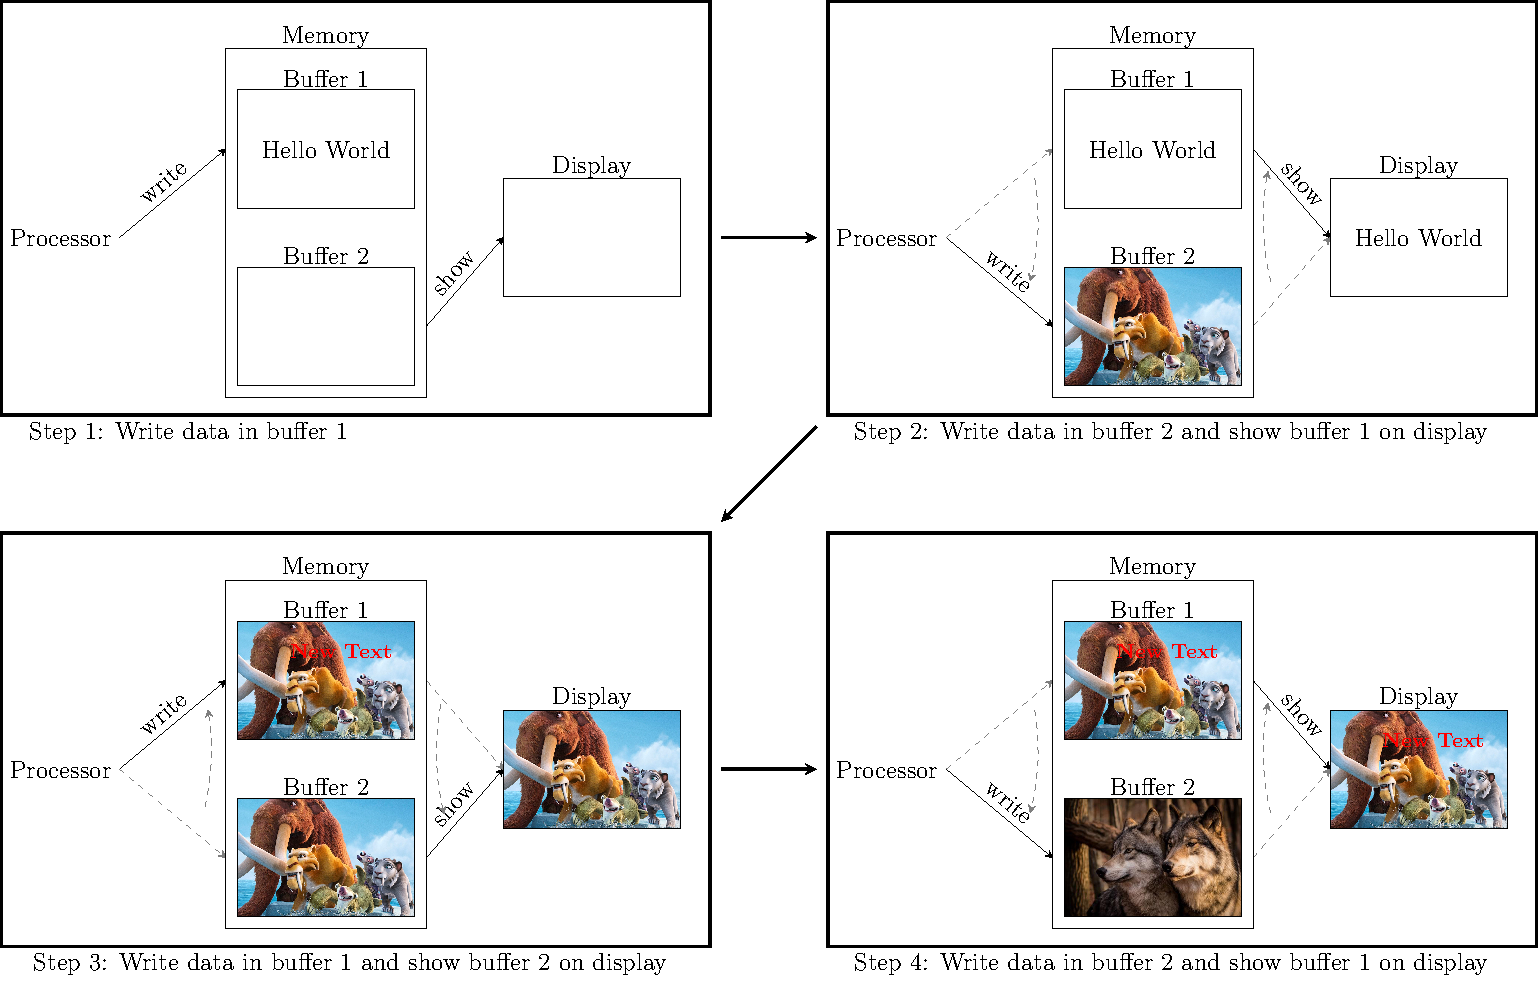
\includegraphics[width=0.9\textwidth]{2-theory/drawing-graphics/graphics/buffer.pdf}
	\caption{Double buffering.\label{theory:buffer}}
\end{figure}

While the new data is written in to one buffer, the screen displays the data located in the other buffer at the same time.

\subsubsection{Compressed fonts}\label{theory:CompressedFonts}
To write a specific character to the display, the controller needs to know how the font is structured.
Figure \ref{theory:font12} shows how the character A could look.
\begin{figure}[ht]
	\centering
	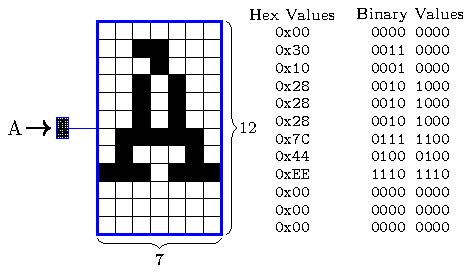
\includegraphics[width=0.8\textwidth]{2-theory/drawing-graphics/graphics/font12.pdf}
	\caption{Creation of a simple seven to twelve pixel sized font.\label{theory:font12}}
\end{figure}
The character is stored this way into the memory and can be accessed just like a look-up table.
If fonts are stored with a $12\times 7$ pixel mask, every character occupies 12 bytes memory.

To display characters in color, 8 more bits for the color depth are needed.
this is visualized in Figure \ref{fig:ganzes_fig}  

\begin{figure}[ht]
	\centering
	\subfigure[1 bit colour font\label{fig:1bitcolor}]{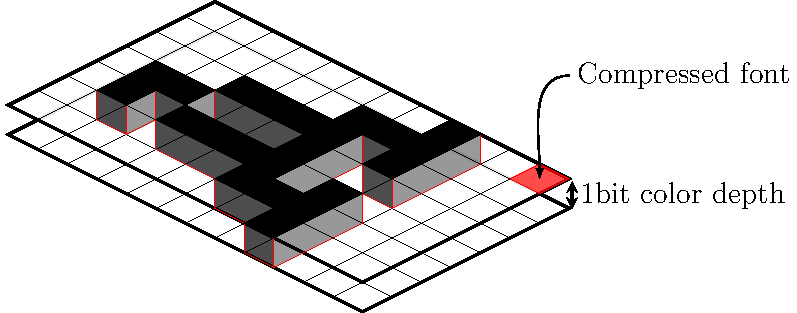
\includegraphics[width=0.49\linewidth]{2-theory/drawing-graphics/graphics/drawingfont.pdf}}
	\subfigure[8 bit colour font (value for blue)\label{fig:Colorblue}]{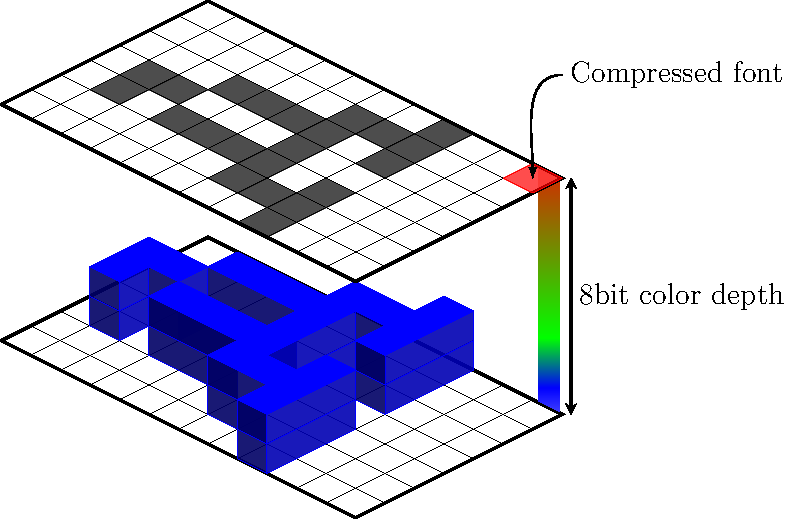
\includegraphics[width=0.49\linewidth]{2-theory/drawing-graphics/graphics/drawingfont8blue.pdf}}
	\subfigure[8 bit colour font (value for green) \label{fig:Colorgreen}]{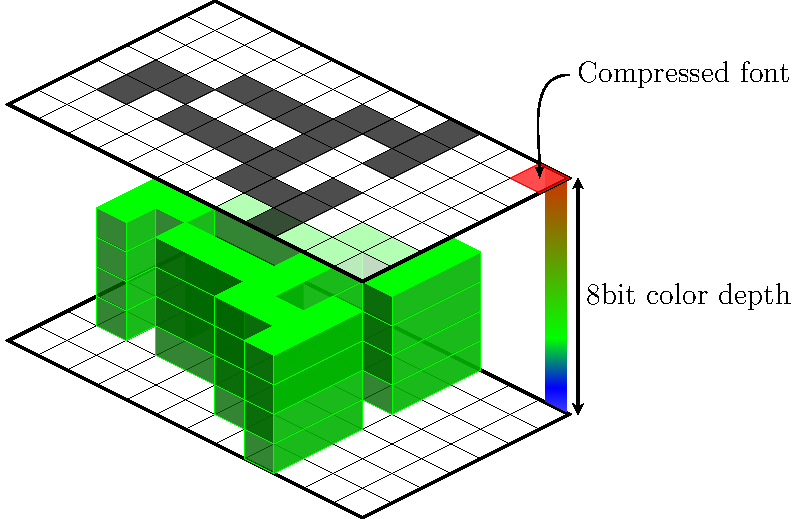
\includegraphics[width=0.49\linewidth]{2-theory/drawing-graphics/graphics/drawingfont8green.pdf}}
	\subfigure[8 bit colour font (value for red) \label{fig:Colorred}]{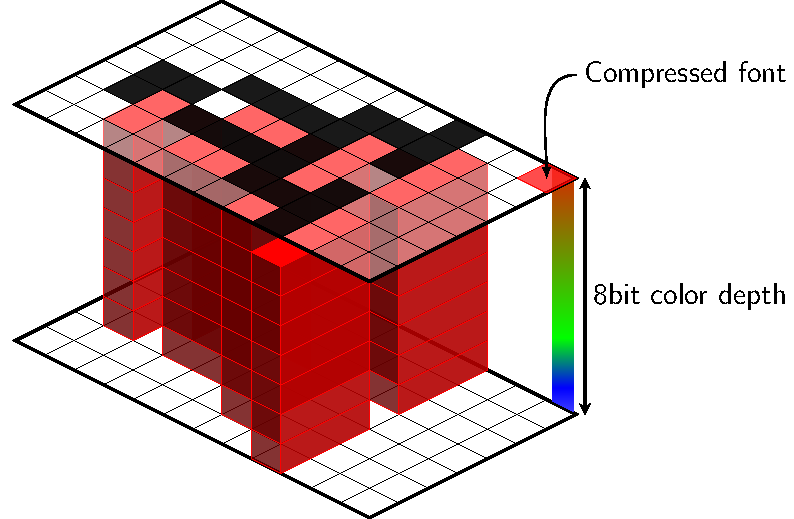
\includegraphics[width=0.49\linewidth]{2-theory/drawing-graphics/graphics/drawingfont8red.pdf}}
	\caption{$12 \times 7$ pixel font mask displayed with $1$- and $8$bit colour depth}
	\label{fig:ganzes_fig}
\end{figure}

%Fig.\,\ref{fig:ganzes_fig}, Fig.\,\ref{fig:a}, Fig.\,\ref{fig:b}, Fig.\,\ref{fig:c}, Fig.\,\ref{fig:d}



\chapter{Evaluation}
This chapter lists the pros and cons of available Technologies.
On this basis was evaluated, which hardware is suitable.

\section{Wakeup Receiver}
In this semester thesis, two different implementations of the wakeup receiver technology were compared.
The AS3933 from AMS and the RFicient from the \acf{fraun} which kindly provided an evaluation kit before the actual release of the product.

\subsection{AS3933}
The AS3933 is a low frequency wakeup receiver, which uses \acs{ask} to modulate a carrier frequency between 15-150\,kHz.
The transmitter sends a manchester encoded, programmable wakeup pattern of length 16 or 32 bit.
If this pattern is detected on the receiver end, a wakeup interrupt is generated.
It is also possible to disable the the pattern decoder to run the chip in a frequency detection mode, where a wakeup interrupt is generated as soon as any pattern on the specified frequency is received.
More important features on the receiver end are:
\begin{itemize}
	\item[-] Receiver sensitivity $80\,\mu\text{V$_{\text{RMS}}$}$
	\item[-] Current consumption in 3-channel listening mode $2.3\,\mu\text{A}$
	\item[-] Operating supply range $2.4\,\text{V}-3.6\,\text{V}$
	\item[-] Three antennas (enables 3D detection)
	\item[-] Channels  individually selective to reduce power consumption
\end{itemize}
The low power consumption makes it possible run the receiver in listening mode below $8.3\,\mu\text{W}$\cite{as3933}.

The demo kit comes with a \acs{gui}, which enables the user to set the parameters as desired and adress the registers directly.
The range of the receiver of about 6\,m as first measurement turns out to be very limited.
Even with a 3db sensitivity boost on the receiver side, it is only possible to detect wakeup events from a distance of 9\,m.
The environment (indoor, outdoor) seems to make no huge difference.

As a result, the limited range makes the AS3933 unusable for the prototype. 

\subsection{RFicient}
The Rficient from the \acs{fraun} uses \acs{ook} to modulate a 868\,MHz signal.
It can either run in pure wakeup mode, where the receiver generates an interrupt as soon as a code is received or a selective mode, where a 16 bit wakeup preamble needs to match the receiver. 
After the preamble is detected, the data rate can be changed to transfer more bits which can be sent over an \acs{spi}-bus to a connected device.
This way, it is possible to transmit data bits after the actual wakeup.
Data rates can be set in a range between $256\,\text{bp/s}-32\,\text{kbp/s}$.
The most important features are:
\begin{itemize}
	\item[-] Receiver sensitivity -80\,dBm
	\item[-] Energy consumption $3\,\mu\text{A}$ at $1.5\,\text{V}$ (data rate 1 kbit/s)
	\item[-] Unidirectional data transfer possible	
\end{itemize}
The power consumption therefore is in listening mode (data rate = 1 kb/s) $4.5\,\mu\text{W}$.

Just as the AS3933, the RFicient demo kit comes with a \acs{gui}, which enables the user to set the important parameters and access the register\cite{rficient}.
First measurements showed that the range of the RFicient is far higher than the range of the AS3933.
It is therefore used in the prototype.
\chapter{Development}

\section{Overview}


\textbf{Not Up To Date Graphic}\\

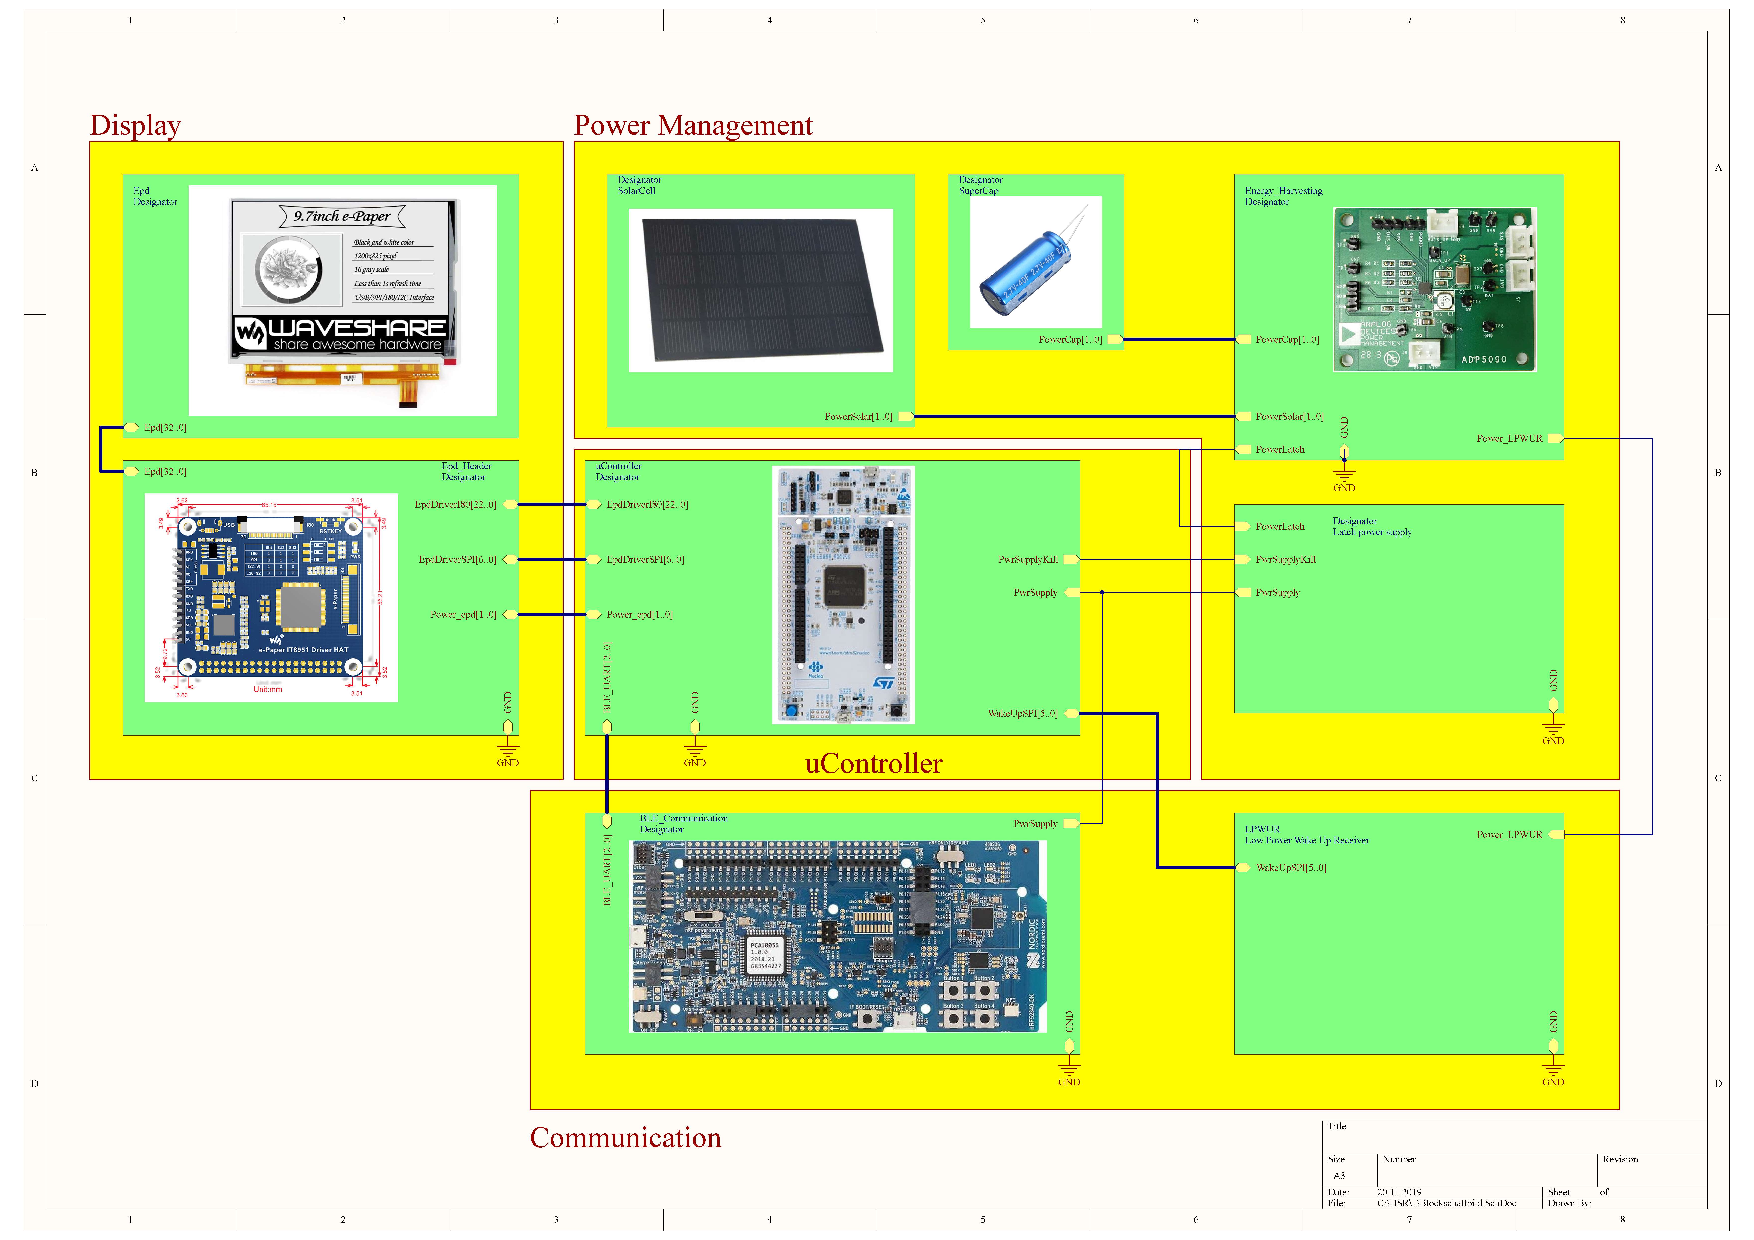
\includegraphics[scale=0.5]{4-development/overview/graphics/Blockschaltbild.pdf}


\section{Hardware}
\begin{figure}[ht]
	\centering
	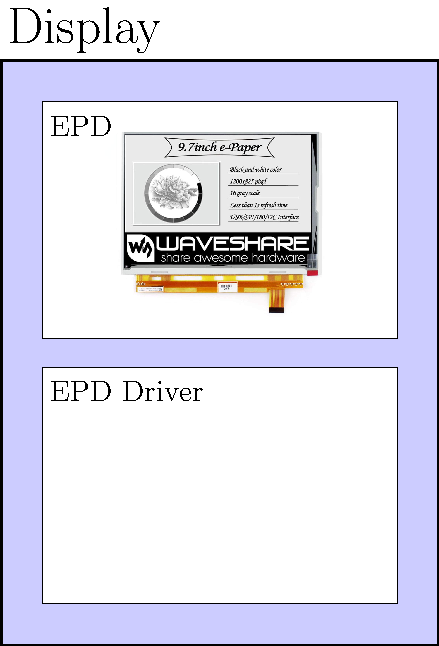
\includegraphics[width=0.9\textwidth]{4-development/hardware/graphics/top/top_schematics.pdf}
	\caption{Receiver schematics\label{hardware:block}}
\end{figure}

\subsection{RFicient}

\subsubsection{Transmitter}
The Rficient demo kit comes, as previously stated with a \acs{gui}.
Is the transmitter module connected, simple steps make it possible to set the preamble and payload data rate. 
The payload itself can partly serve as an ID and as additional transmitted data.
The power of the transmission can also be set between -30\,dBm and 10\,dBm.
The transmitter-\acs{gui} is shown in figure \ref{development:tx}.
\begin{figure}[ht]
	\centering
	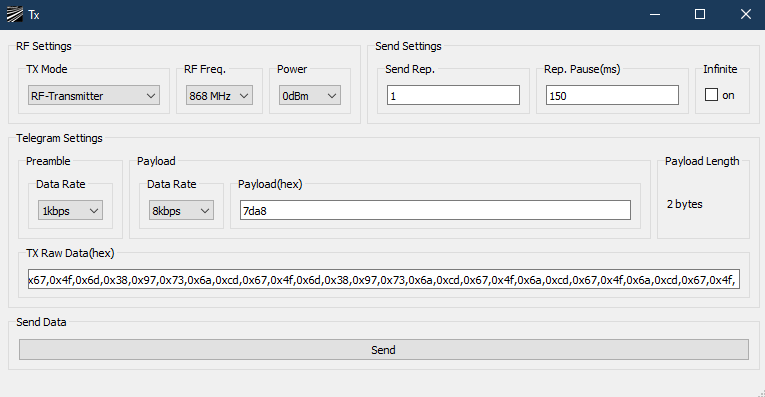
\includegraphics[width=0.9\textwidth]{4-development/hardware/graphics/TXgui.png}
	\caption{Transmitter GUI\label{development:tx}}
\end{figure}
To test, if any data is received, it is helpful to activate the infinite loop (top right in figure \ref{development:tx}).
The defined data is in this case sent repeatedly with an adjustable period.

\subsubsection{Receiver}
To receive the data, the setting of the receiver module need to be matched to the transmitter.
The provided receiver-\acs{gui} makes this step very simple.
As visible in figure \ref{development:rx}, one can enable the four possible interrupt sources: CodeA/B, ID, FIFO length and FIFO overflow.
In the finished product, it should be possible to wake up the receivers individually.
For this reason, only the ID as interrupt source is of interest.
\begin{figure}[ht]
	\centering
	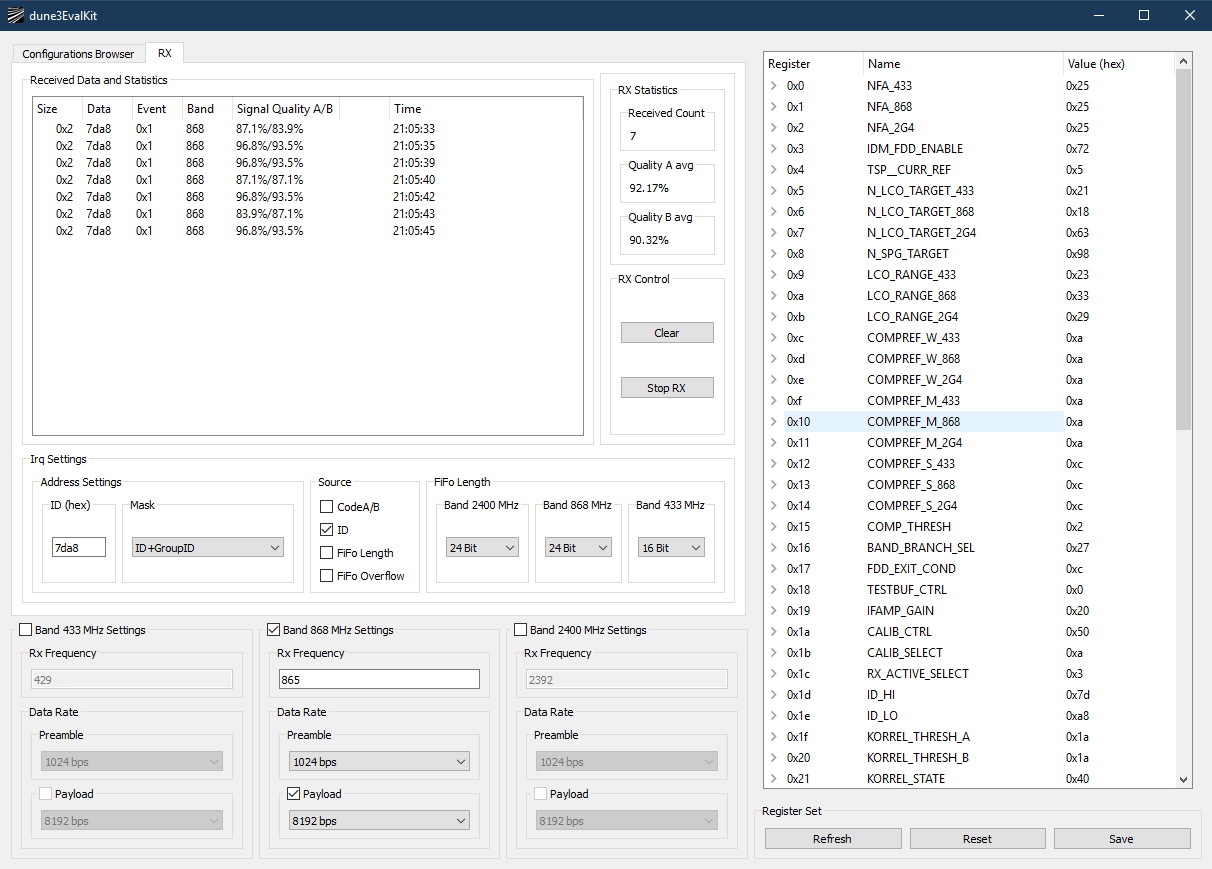
\includegraphics[width=0.9\textwidth]{4-development/hardware/graphics/RXgui.png}
	\caption{Receiver GUI\label{development:rx}}
\end{figure}
If an interrupt is generated, the RFicient sets a \acs{gpio}-pin to high, and transfers the received data to a \acs{fifo}-buffer.
This data can be passed to a microcontroller over an \acs{spi}-bus.
For the purpose of this thesis, only the \acs{gpio} high level is used as a on switch of a self-holding circuit.

\subsubsection{Tests in a realistic environment}
To test the RFicient in more detail, some indoor measurements were made.
As test environment served several buildings of the \acf{hsr}, since this type of facility represents a realistic condition for the developed schedule.

Purpose of the first test was to measure the achievable range.
Figure \ref{development:env1} shows the hallway where this test was executed.
\begin{figure}[ht]
	\centering
	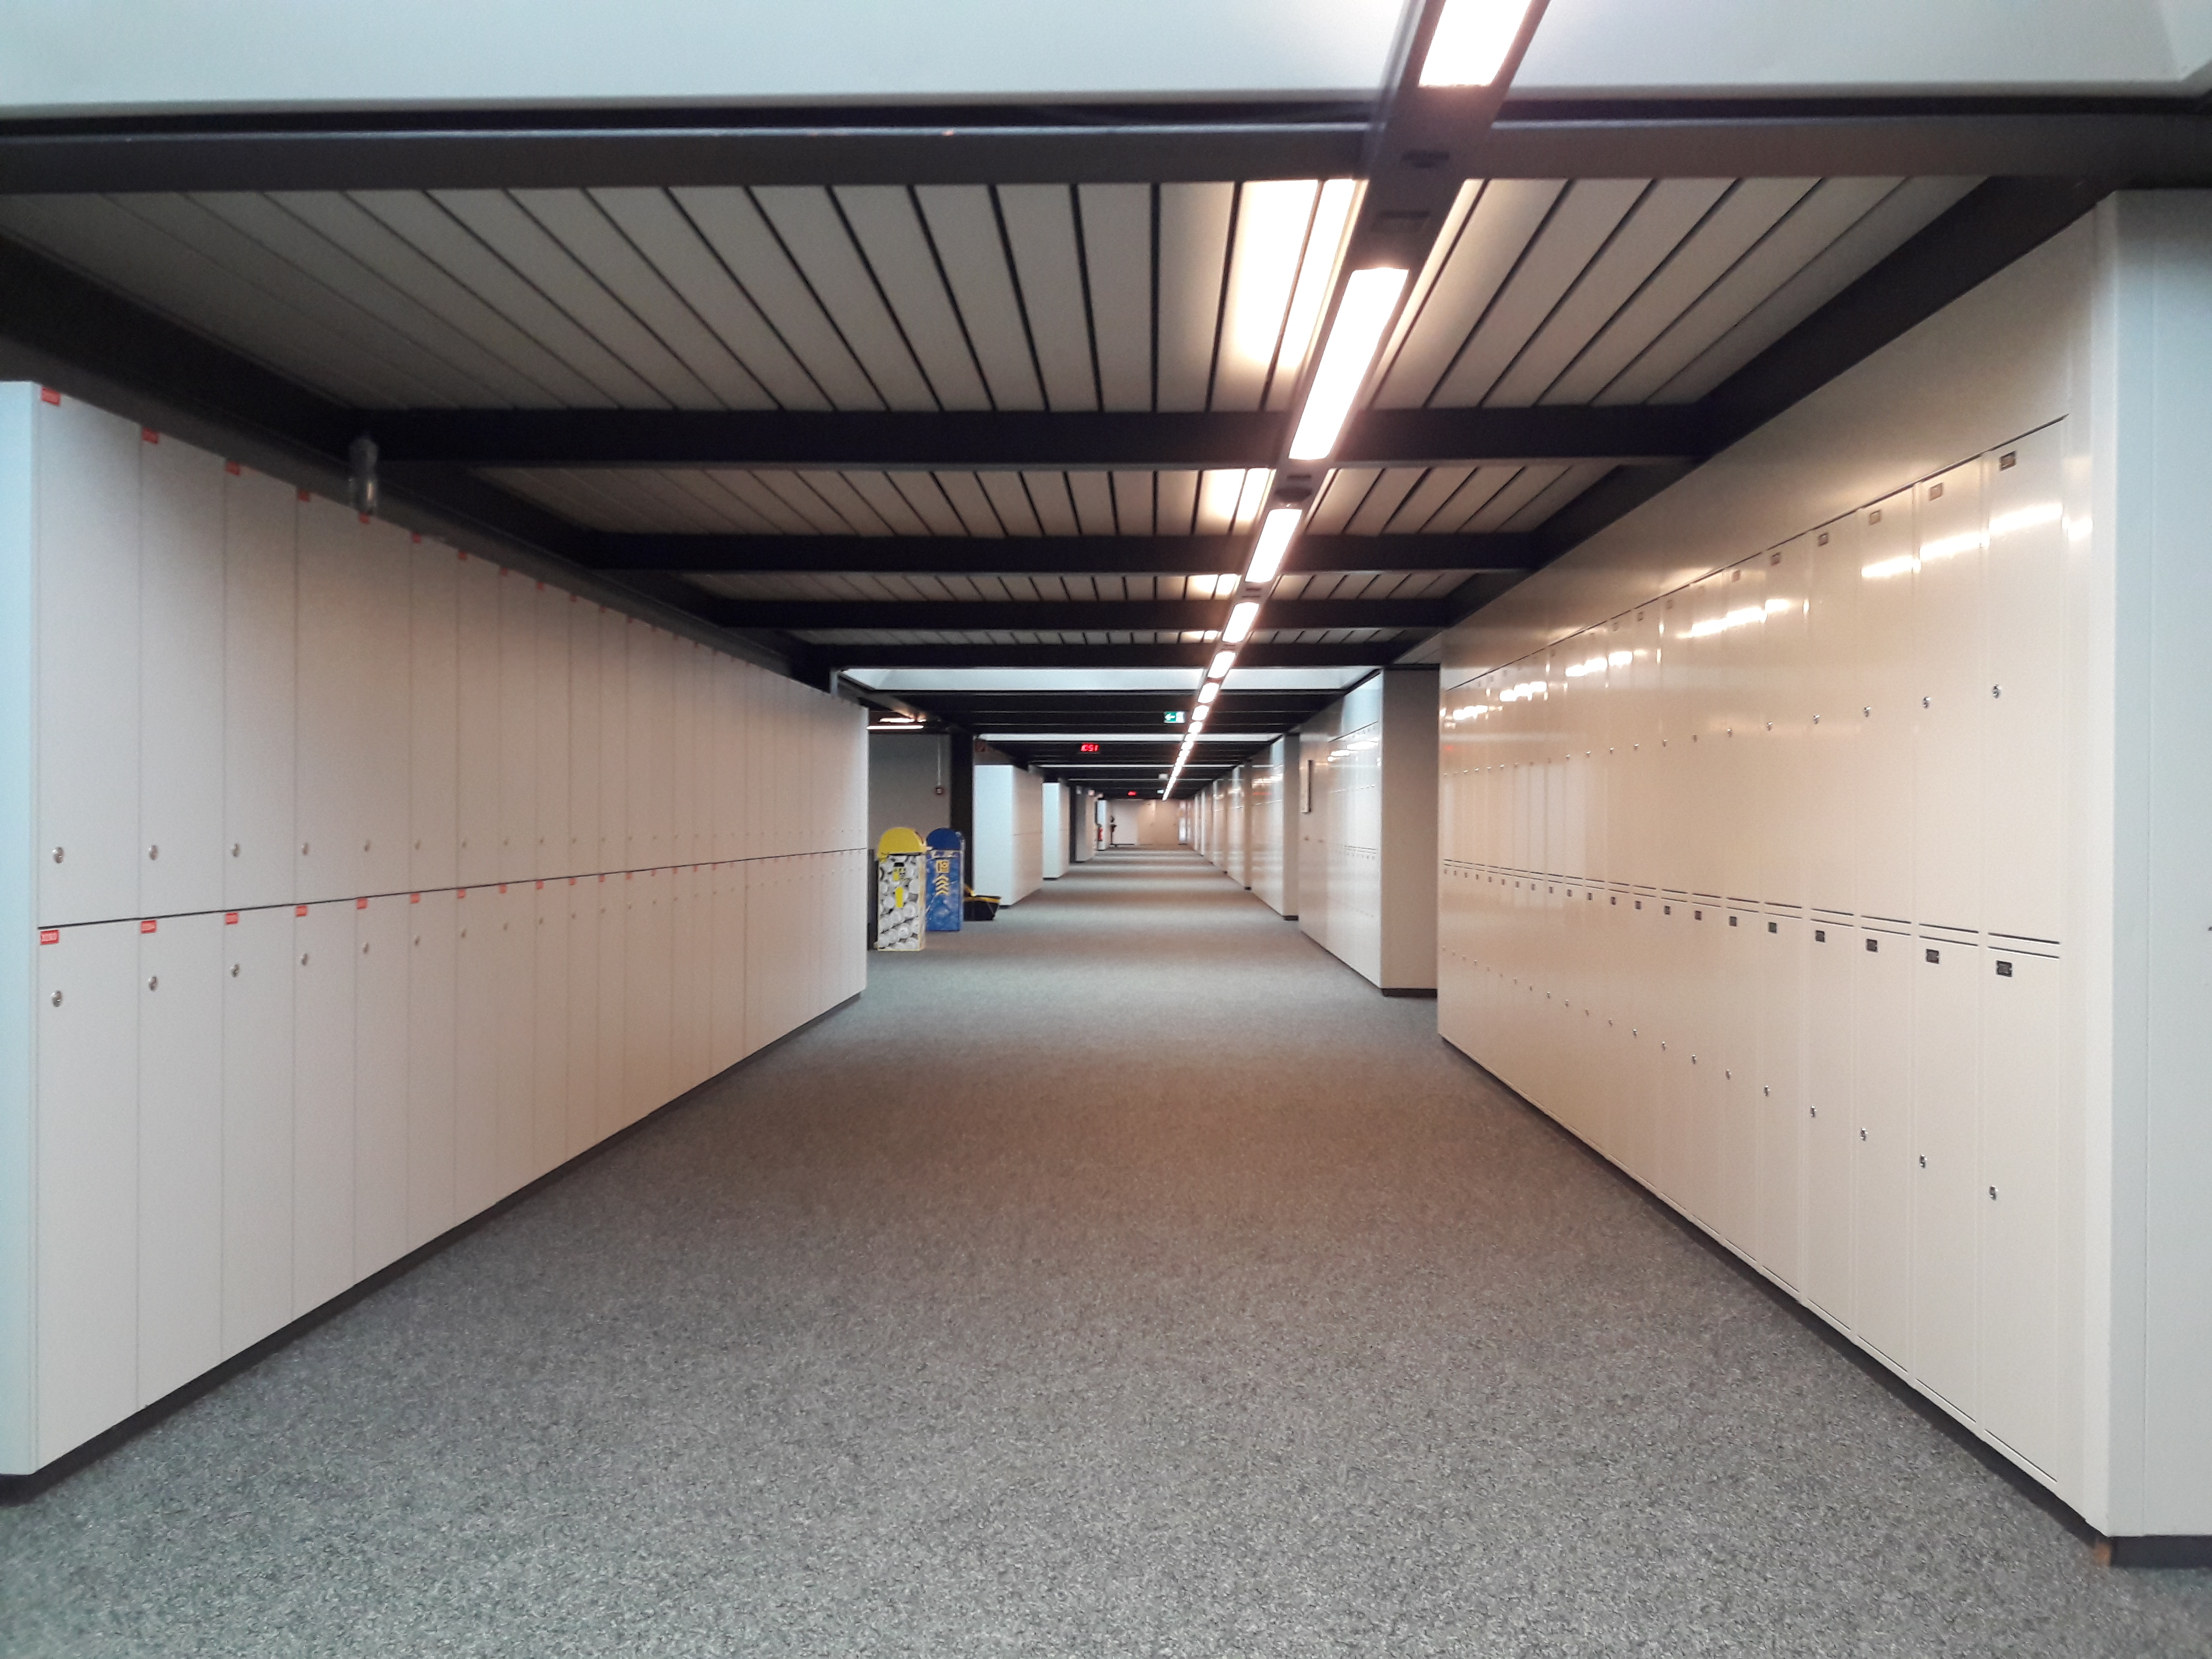
\includegraphics[width=0.9\textwidth]{4-development/hardware/graphics/env1.jpg}
	\caption{Test environment 1 (\acs{hsr} building 1)\label{development:env1}}
\end{figure}
With a transmission power of 0\,dBm (1\,mW) it is possible to receive interrupt over a 50\,m distance (line of sight).
Is the transmission power increased to 10\,dBm (10\,mW), interrupts can be sent over a distance up to 80\,m.
In this environment, the Rficient has enough range.
But maybe reflections off the walls, floor and ceiling have contributed to this result.

Out if this reason, a second test was performed to check how the RFicient penetrates obstacles.
As test environment served this time the \acs{hsr} builing 8, as depicted in figure \ref{development:env2}.
An attempt was made to send wakeup signals through the ceiling.
\begin{figure}[ht]
	\centering
	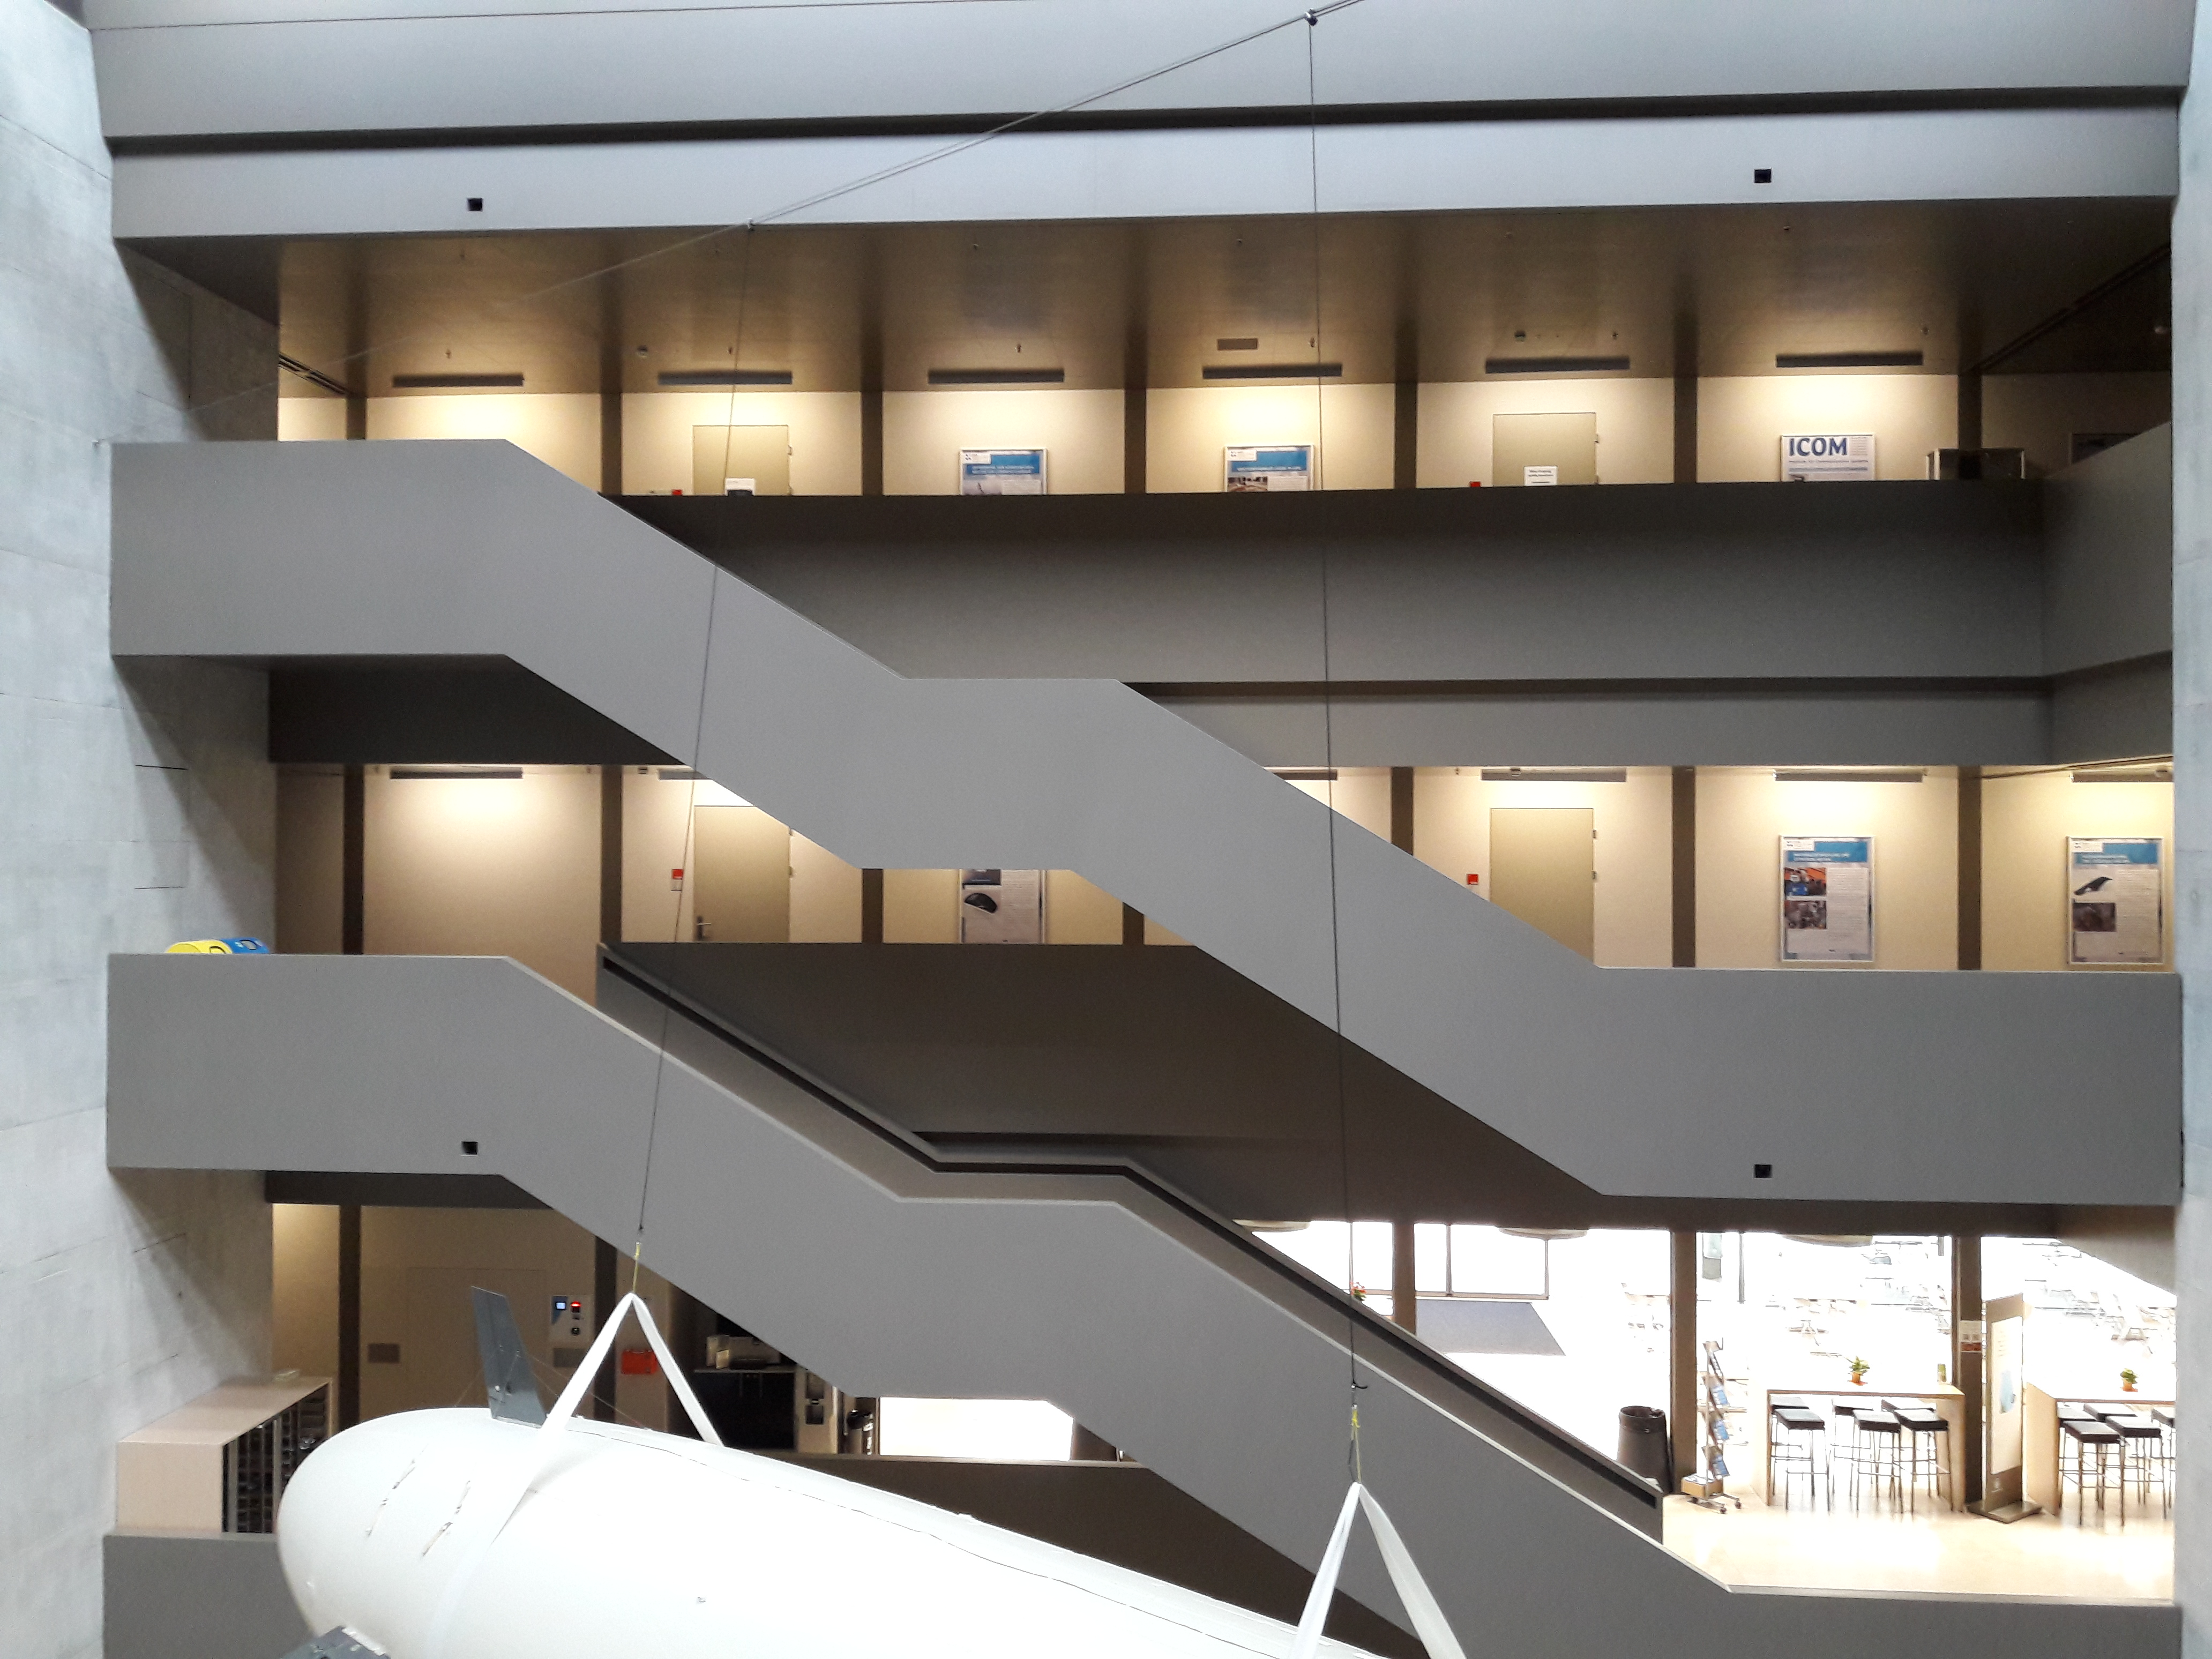
\includegraphics[width=0.9\textwidth]{4-development/hardware/graphics/env2.jpg}
	\caption{Test environment 2 (\acs{hsr} building 8)\label{development:env2}}
\end{figure}
To avoid reflections, the RFicient was placed in such a way, that the zero point of the antenna pointed directly at the opposite walls.
With a transmisson power of 0\,dBm, two ceilings can be penetrated.
Is the power again increased to 10\,dBm, the signal reached through three ceilings.

These measurements further confirmed, that the RFicient is suitable for the use-case of this semester thesis.

\subsection{Energy Harvesting}
The screen should be self-sustaining, thus some sort of energy-harvesting unit is needed.
It was apparent to choose light as the energy source, since the screen will be used in rooms, that are artificially illuminated most of the time.
The energy  obtained by solar cells is converted to a suitable voltage, using a ADP5090 chip.
This way, a super-capacitor, which is used as an energy storage device, is charged.

\subsubsection{Solar cell}
As solar cell, the AM-1522 by Panasonic is used.
One panel has an area of $55.0\,\text{mm}\,\times\,40.5\,\text{mm}$ and delivers up to $58.7\, \mu\text{A}$ when operating at an optimal voltage of $2.1\,\text{V}$, provided an illuminance of 200\,lux.
To keep a reasonable display to panel ratio, four cells where connected in parallel, which corresponds to an area of ca. $89.1\,\text{cm}^2$ (Display area = $283\,\text{cm}^2$). Therefore, the solar cells should provide a power of

\begin{align}
	P = U\cdot I = 4\cdot 57.8\,\mu\text{A}\cdot 2.1\ \text{V}=485.52\,\mu \text{W},\label{development:cell_power}
\end{align}

given a 200 lux illuminance \cite{amorton}.

\subsubsection{Power management}
The ADP5090 from Analog Devices is used on the power management.
This boost regulator makes it possible to charge storage elements, such as rechargeable batteries and super capacitors with the input dc-power provided by the PV-cell. Utilized features are:
\begin{itemize}
	\item[-] Maximum power point tracking
	\item[-] Efficiency up to 90\%
	\item[-] Input voltage $V_{IN}$ from $80\,\text{mV}$ to $3.3\,\text{V}$
	\item[-] Programmable voltage range ($2.2\,\text{V}$ to $5.2\,\text{V}$) for the storage element
\end{itemize}
To prevent the storage element from overdischarging, the ADP5090 enables the user to set a maximal Voltage with resistors:

\begin{align}
	V_{\text{BAT\_TERM}} = \frac{3}{2} V_{\text{REF}}\left(1+\frac{R_{\text{TERM1}}}{R_{\text{TERM2}}} \right).\label{development:v_bat_term} 
\end{align} 

The same procedure is applied to set a minimal voltage:

\begin{align}
	V_{\text{BAT\_SD}}=V_{\text{REF}} \left(1+\frac{R_{\text{SD1}}}{R_{\text{SD2}}} \right).\label{development:v_bat_sd} 
\end{align}  

While discharging, the ADP5090 will switch off the output $V_{\text{SYS}}$ if $V_{\text{BAT\_SD}}$ is reached. This prevents the storage element from overdischarging.
The output voltage $V_{\text{SYS}}$, where the load is attached, will therefore always stay in this programmed range $(V_{\text{BAT\_SD}}\le V_{\text{SYS}}\le V_{\text{BAT\_TERM}})$ \cite{adp}.

For this prototype, the evaluation board for the ADP5090 was used, where the internal reference voltage ($V_{\text{REF}}$ in \eqref{development:v_bat_term} and \eqref{development:v_bat_sd}) is $1.21\,\text{V}$ \cite{adp_eval}.

\subsubsection{Super capacitor}
As energy storage, a super capacitor from Taiyo Yuden (LIC1235RS3R8406) has proven to be suitable, which is a $40\,\text{F}$ cylinder type lithium ion capacitor.
The operating voltage range is between $2.2\,\text{V}$ and $3.8\,\text{V}$.
Discharging the capacitor lower than $2.2\,\text{V}$ causes shorter lifetime and higher leakage current.
The same unwanted behaviour occurs when charging the capacitor over $3.8\,\text{V}$ \cites{yuden}.

\subsubsection{Combined test}
To test the behaviour of the power management, supercapacitor and solar cells, a couple of measurements are executed.
Figure \ref{development:test} shows the layout of the test setup.

\begin{figure}[ht]
	\centering
	
\includegraphics[width=0.9\textwidth]{4-development/hardware/graphics/testaufbau.pdf}
	\caption{Schematics of the test setup\label{development:test}}
\end{figure}

To carry out these measurements, it is first necessary to adjust the minimal and maximal voltage of the ADP5090.
The nrf58240 accepts supply voltages between $1.6\,\text{V}$ up to $5.5\,\text{V}$ \cite{nrf}.
The STM32 on the other side is less flexible with an input voltage range of $1.71\,\text{V}$ to $3.6\,\text{V}$ \cite{stm32}.
As stated in the section above, the super capacitors operating voltage is between $2.2\,\text{V}$ and $3.8\,\text{V}$.
Hence it seems reasonable, to set $V_{\text{BAT\_TERM}} \le 3.6\,\text{V}$ and $V_{\text{BAT\_SD}} \ge 2.2\,\text{V}$, to satisfy all of these three elements.
In order to do this, the four resistors have to be chosen as $R_3 = 4.3\,\text{M}\Omega$, $R_6 = 4.7\,\text{M}\Omega$, $R_2 = 4.3\,\text{M}\Omega$ and $R_3 = 5.1\,\text{M}\Omega$.
Inserted in the equation \eqref{development:v_bat_term} and \eqref{development:v_bat_sd} we get
\begin{align}
	V_{\text{BAT\_TERM}}= \frac{3}{2} 1.21\,\text{V} \left(1 + \frac{4.3\,\text{M}\Omega}{4.7 \,\text{M}\Omega} \right) \approx 3.48\,\text{V} 
\end{align}
and
\begin{align}
	V_{\text{BAT\_SD}} = 1.21\,\text{V} \left(1 + \frac{4.3\,\text{M}\Omega}{5.1\,\text{M}\Omega} \right) \approx 2.23\,\text{V}. 
\end{align}

While testing, the input voltage from the solar cells ($V_{\text{IN}}$), voltage of the supercap ($V_{\text{BAT}}$) and the output voltage ($V_{\text{SYS}}$) are tracked. Additionally, the illuminance ($E_\text{v}$) near the PV-cells  is recorded as indicated in figure \ref{development:test}.

The purpose of the first test is to check, if the ADP5090 converts $V_{\text{IN}}$ to a voltage $\le V_{\text{BAT\_TERM}}$.
The measurements where taken over a couple hours and are plotted in Figure \ref{development:charge}.

\begin{figure}[ht]
	\centering
	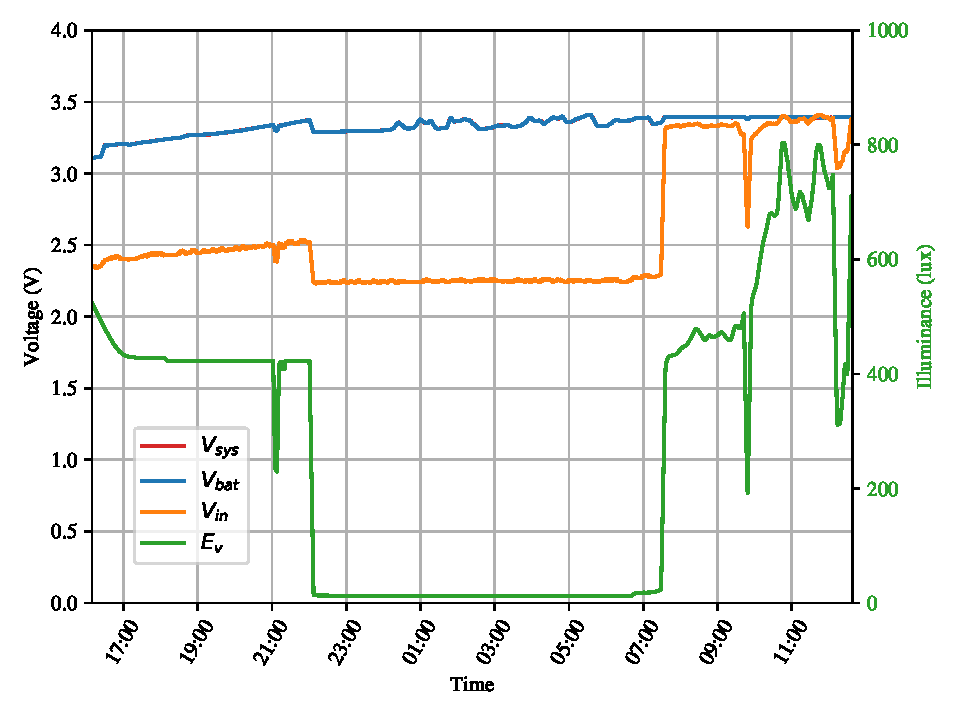
\includegraphics[width=0.9\textwidth]{4-development/hardware/graphics/laden.pdf}
	\caption{Charging behaviour\label{development:charge}}
\end{figure}

No load was connected to the output ($Z_\text{LOAD} \to \infty$), which is the reason $V_{\text{SYS}}$ is overlapped by $V_{\text{BAT}}$.
It can be seen, that between 17:00 and 23:00, the super capacitor was being charged and
that the ADP5090 controls the voltage $V_{\text{BAT}}$ like expected to the adjusted maximum voltage $V_{\text{BAT\_TERM}}$.

The second test should simulate the discharging when a load is connected, after the capacitor was fully charged.
It was necessary to estimate the consumed power by the electronic components of the prototype.
A rough measurement with a power analyser showed, that the microcontroller and the e-paper display together draw at its peak about $240\,\text{mA}$ when connected to $5\,\text{V}$. The nrf52840 on the other hand, only consumes 6 mA with a 3 V source. Thus the expected consumed power at is's peak is:
\begin{align}
	P_{e} = 5\,\text{V}\cdot 0.24\,\text{A} + 3\,\text{V}\cdot 0.006\,\text{A} = 1.218\,\text{W}.
\end{align}
  

If $Z_{\text{LOAD}}=10\,\Omega$ the load draws currents between $0.223\,\text{A}$ and $0.348\,\text{A}$ which again lead to a power consumption that should approximately match the power consumption of the finished prototype.
Furthermore, the solar cells where covered to observe the discharging without interference of additionally charging behaviour.
Figure \ref{development:discharge} shows the result.
 
\begin{figure}[ht]
	\centering
	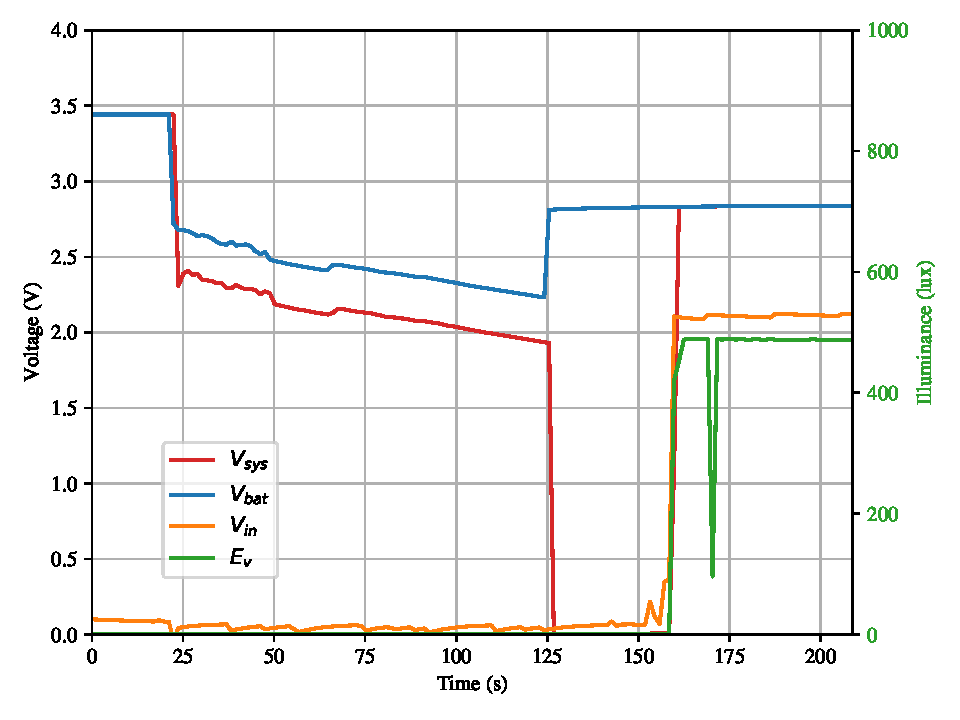
\includegraphics[width=0.9\textwidth]{4-development/hardware/graphics/entladen.pdf}
	\caption{Discharging behaviour\label{development:discharge}}
\end{figure}

As soon as the load is connected (after 25\,), $V_{\text{SYS}}$ and $V_{\text{BAT}}$ first drop by almost $1\,\text{V}$ and after that steadily decrease.
After ca. 100 s, $V_{\text{BAT}}$ reached the value of $V_{\text{BAT\_SD}}$ and the ADP5090 switches the output off ($V_{\text{SYS}}$ drops to 0) to prevent the capacitor from overdischarging.
The output now stays switched off, until $V_{\text{IN}}$ again supplies energy, and $V_{\text{BAT}} \le V_{\text{BAT\_SD}}$.
It can also clearly be seen, that after 160 seconds, the ADP5090 controls $V_{\text{IN}}$ to ca. $2.1\,\text{V}$. Recall that this is the optimal power point of the solar cell.


\newpage
\section{Software}
\begin{figure}[H]
	\centering
	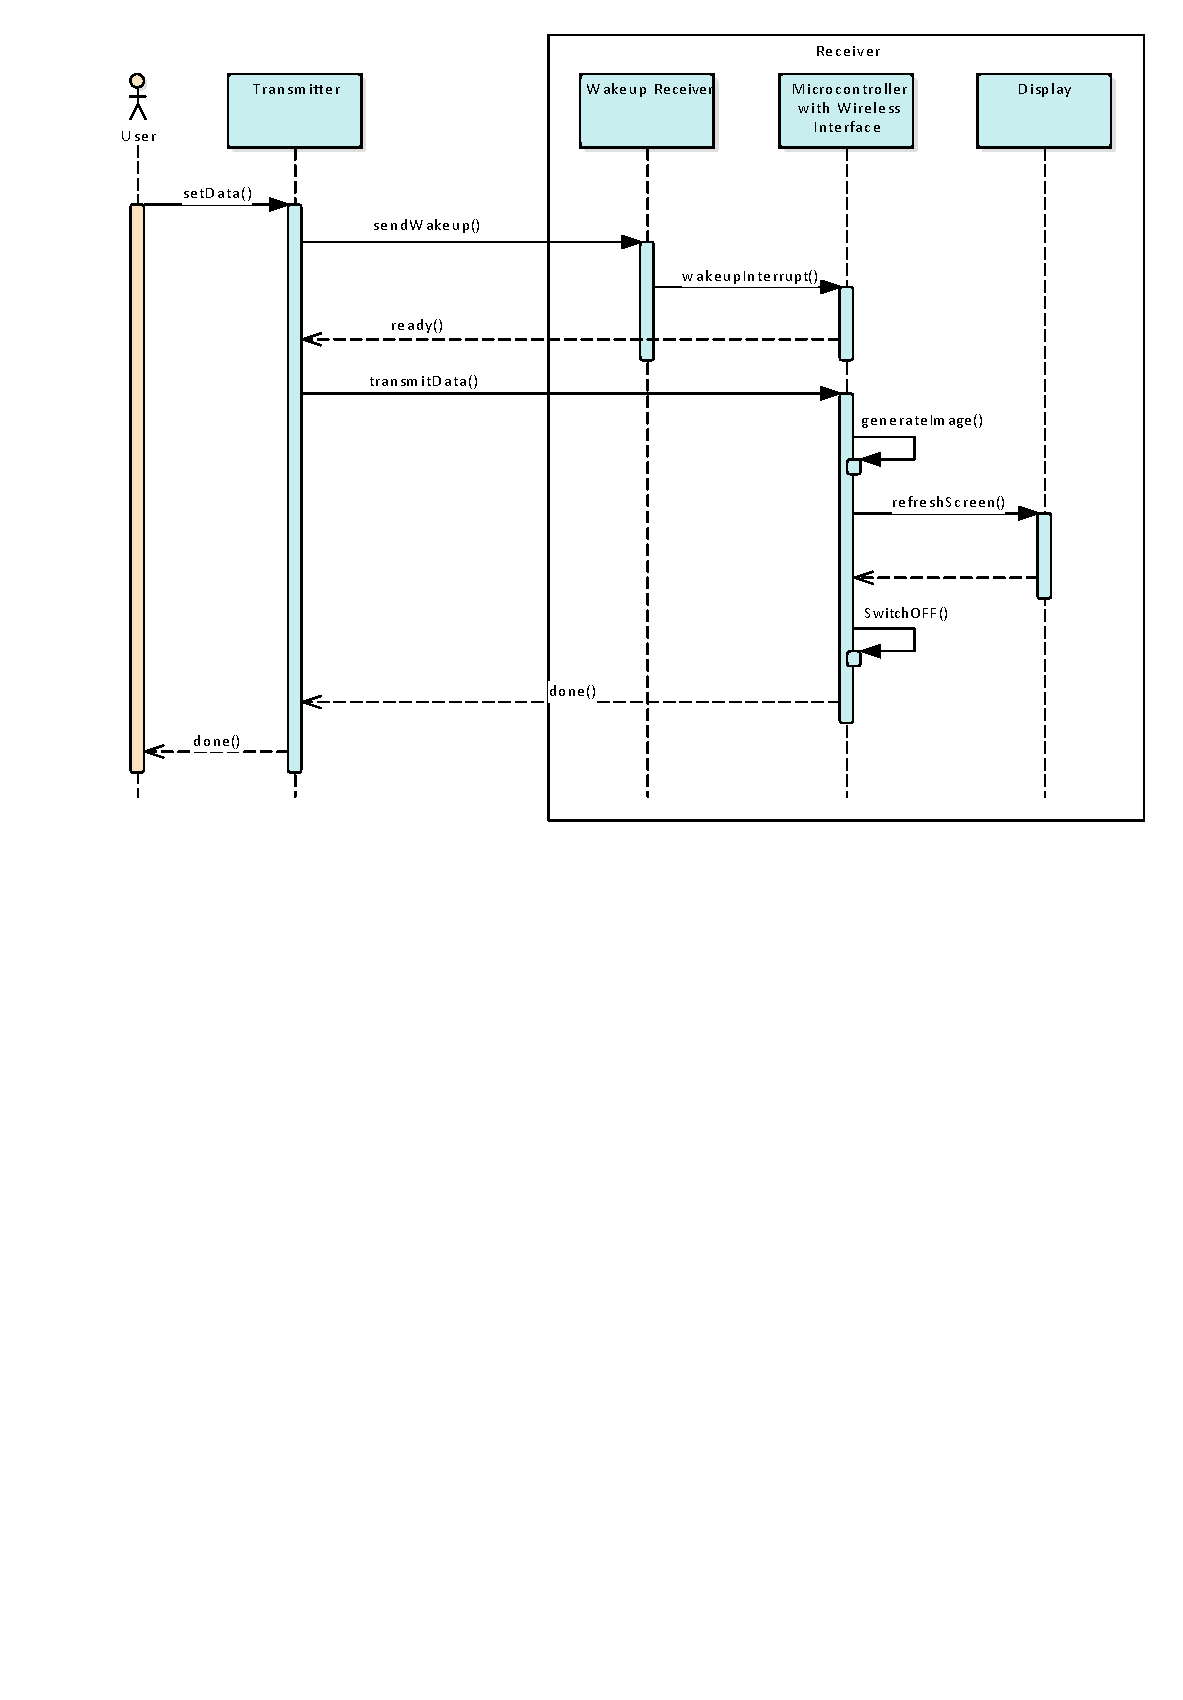
\includegraphics[width=0.9\textwidth]{4-development/software/graphics/sequence.pdf}
	\caption{not up to date sequence\label{software:sequence}}
\end{figure}


\subsection{Receiver}


\subsubsection{Microcontroller}
The main controller of the receiver is the STM32. To develop firmware for the microcontroller the Hardware abstractions layer provided by STMicroelectronics is used. The firmware running on the STM32 is responsible for the following tasks:
\begin{itemize}[H]
	\item[-] Initialize the IT8951 display driver chip
	\item[-] Receive data via UART from the BLE module
	\item[-] Generating the displayed image data from a template
	\item[-] Writing received text strings to the EPD
	\item[-] Writing the image data to the display driver via SPI
	\item[-] Control the power supply of all the different components
\end{itemize}
\paragraph{Configurations}

\begin{center}
	\begin{tabular}{ |c|c|c|c|c| } 
		\hline
		Description & Function &Pin number & Speed& Properties \\
		\hline
		\multirow{4}{4em}{SPI} 	& Chip select & PA0& &No Pull-up/-down \\ 
								& Clock& PA1 & 14.0 MBits/s&No Pull-up/-down \\ 
								& MISO & PA6&14.0 MBits/s & No Pull-up/-down  \\ 
								& MOSI & PA7& 14.0 MBits/s&No Pull-up/-down  \\ 
		\hline
		\multirow{2}{4em}{UART} & TX & PC10 & 115.2 kBits/s & Pull-up   \\ 
								& RX & PC11 & 115.2 kBits/s & Pull-up \\ 
	\hline
	\end{tabular}
\end{center}
\begin{figure}[H]
	\centering
	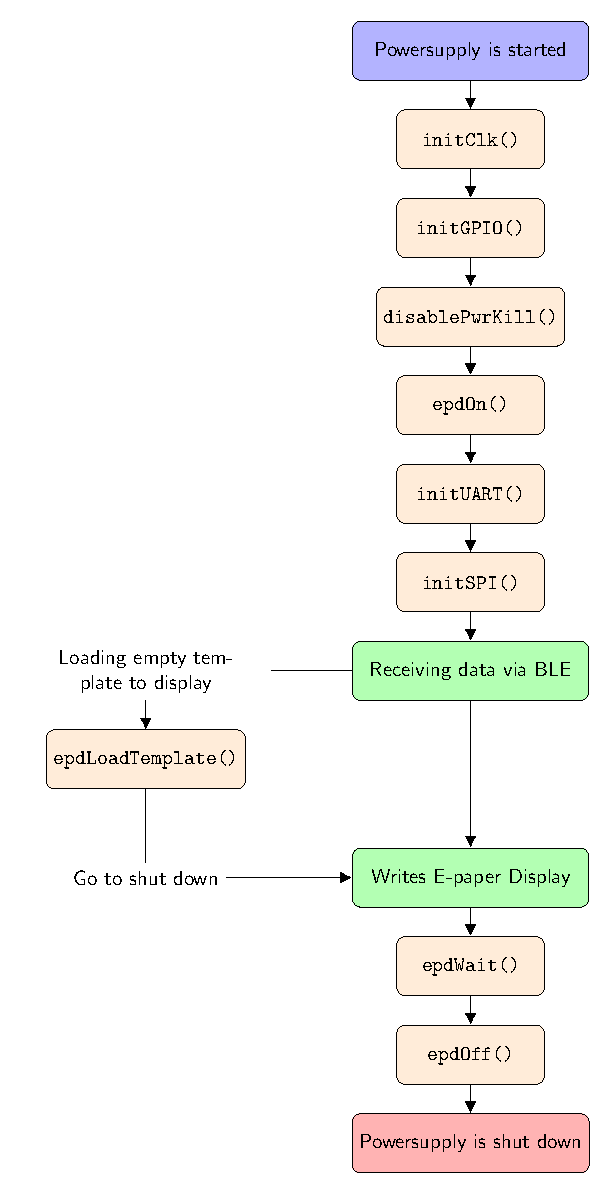
\includegraphics[height=0.8\textheight]{4-development/software/graphics/main.pdf}
	\caption{STM32 program flow chart\label{software:main}}
\end{figure}
In the flowchart\ref{software:main} it is visible that the controller itself never enters a deep sleep mode in the end of an program cycle. Instead the controller runs trough a power kill sequence which disables the own power supply. As a result of this the controller and remaining hardware consume no power instead of their deep sleep power consumption. 

\paragraph{Template}
The calendar template is getting preloaded in the flash of the STM32. To save memory, the file is converted into an $1200 \times 825$ PNG with the colour depth of 4 bit. The PNG then is used to create a .c file which holds an one dimensional array with all the pixel data in it.

\paragraph{Writing characters}
\lstdefinestyle{mystyle}{
	language=c,
	tabsize=4,
	showstringspaces=false,
	backgroundcolor = \color{gray!15!white},
	basicstyle=\scriptsize\ttfamily,
	morekeywords={as},
	keywordstyle=\color{red!80!black},
	stringstyle=\color{green!50!black},
	numberstyle=\color{red},
	emph={int,char,double,float, uint8_t, uint16_t},
	emphstyle=\color{green!50!black}
}
\lstset{style=mystyle}

\begin{figure}[ht!]
	\begin{lstlisting}
void drawChar(uint16_t Xpt, uint16_t Ypt, const char Acsii_Char,
					sFONT* Font, uint8_t cBackground, uint8_t cForeground)
	{
		uint16_t Page, Column;
		if (Xpt > Paint.Width || Ypt > Paint.Height) 
		{
			return;
		}
	uint32_t Char_Offset = (Acsii_Char - ' ') * Font->Height * 
							(Font->Width / 8 + (Font->Width % 8 ? 1 : 0));
	const unsigned char *ptr = &Font->table[Char_Offset];
	
	for (Page = 0; Page < Font->Height; Page ++ ) 
	{
		for (Column = 0; Column < Font->Width; Column ++ ) 
		{
			if (FONT_BACKGROUND == cBackground) 
			{ 
				if (*ptr & (0x80 >> (Column % 8)))
					Paint_SetPixel(Xpt+Column, Ypt+Page, cForeground);
			} 
			else 
			{
				if (*ptr & (0x80 >> (Column%8))) 
				{
					Paint_SetPixel(Xpt + Column, Ypt + Page, cForeground);					
				} 
				else 
				{
					Paint_SetPixel(Xpt + Column, Ypt + Page, cBackground);
				}
			}
			//One pixel is 8 bits
			if (Column % 8 == 7)
				ptr++;
		}
		if (Font->Width % 8 != 0)
			ptr++;
	}
}
	\end{lstlisting}
\end{figure}
\begin{figure}[ht!]
\begin{lstlisting}
void drawString(uint16_t xStart, uint16_t yStart,const char * pString, sFONT* Font,
							 uint8_t cBackground,uint8_t cForeground) 
{
	uint16_t Ypt = yStart;
	uint16_t Xpt = xStart;
	
	if (xStart > Paint.Width || yStart > Paint.Height)
	{
		return;
	}
	while (* pString != '\0') 
	{
		if ((Xpt + Font->Width ) > Paint.Width ) 
		{
			Xpt = xStart;
			Ypt += Font->Height;
		}
		if ((Ypt  + Font->Height ) > Paint.Height ) 
		{
			Xpt = xStart;
			Ypt = yStart;
		}
		Paint_DrawChar(Xpt, Ypt, * pString, Font, cBackground, cForeground);
		pString ++;
		Xpt += Font->Width;
	}
}	
\end{lstlisting}
\end{figure}


\subsubsection{Communication}
The software on both sides of the bluetooth channel is very similar, thus it is explained in this section.
A \acs{ble} example project, which was provided by nordic, was only slightly changed to fit the purpose of this prototype.

Before a connection is established, the module on the receiver side is known as peripheral, and the module on transmitter end as the central device.
After the receiver is woken up with the RFicient, the peripheral starts advertising.
Advertising basically means sending data packets periodically with information for the central device.
The central is scanning for the this advertisement and can based on this information decide, if it wants to connect.
Is the connection established, it is now possible to exchange data through this channel.
This process is illustrated in Figure \ref{software:ble}.
\begin{figure}[ht]
	\centering
	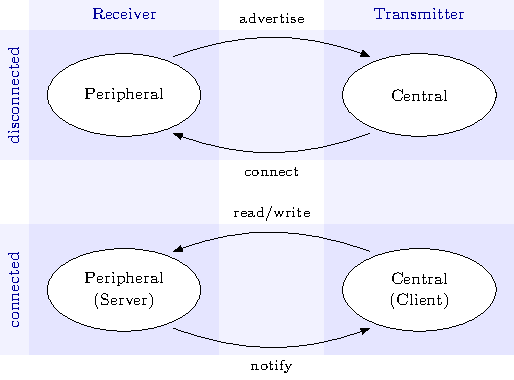
\includegraphics[width=0.8\textwidth]{4-development/software/graphics/ble.pdf}
	\caption{\acs{ble}-communication with the nRF52480.\label{software:ble}}
\end{figure}

The central serves after connection as the client.
It can make read and write requests to access the data on the peripheral, which acts as the server.
The server on the other hand can only send notifications to the client if new data is ready.
It should be noted, that the roles of client and server do not in any case have to be assigned to central and peripheral, but also the other way around. 

\subsection{Transmitter}

\subsubsection{Python-Script}
\lstset{basicstyle=\footnotesize}
\lstdefinestyle{mystyle}{
	language=Python,
	tabsize=4,
	showstringspaces=false,
	backgroundcolor = \color{gray!15!white},
	basicstyle=\scriptsize\ttfamily,
	morekeywords={as},
	keywordstyle=\color{blue!50!black},
	stringstyle=\color{green!50!black},
	numberstyle=\color{red},
	emph={int,char,double,float,range, len, bytes},
	emphstyle=\color{violet}
}
\lstset{style=mystyle}

A short python script enables the user to send the data to the display.
This script is looked at here step by step.

\begin{enumerate}
	\item Include of the used packages, time and serial.
	\begin{lstlisting}
	import serial
	import time
	\end{lstlisting}	
	\item Set desired baudrate, select which COM-port windows assigned to the development kit and open the port.
	\begin{lstlisting}
	baudrate = 115200
	com_port = 'COM14'
	
	device = serial.Serial(com_port, baudrate, writeTimeout=0)
	\end{lstlisting}
	\item Create a list of list with the desired data.
	The first list contains information about how many packages are about to follow.
	The following list contain the location on the template, the subject and the lecturer.
	\begin{lstlisting}
	data = [[0, chr(3), '\0\0\0\0'],[11 , 'WsComm\0', 'MAH\0'],
			[3 , 'DigPro\0', 'SCU\0'], [22 , 'EmbSW\0', 'BON\0']]
	\end{lstlisting}
	\item Fill the list with \lstinline|'\0'| so every package is 20 bytes long.
	\begin{lstlisting}
	for i in range(len(data)):
		if len(data[i][1])<16:
			t = 14-len(data[i][1])
			data[i][1] = data[i][1]+'\0'*t
	\end{lstlisting}
	\item Store time when data transfer is started.
	\begin{lstlisting}
	t_start = time.time()
	\end{lstlisting}
	\item Transfer data to the nRF52480 transmitter
	\begin{lstlisting}
	for i in range(len(data)):
		device.write([data[i][0]]) 
		device.write(bytes(data[i][1], 'utf-8'))       
		device.write(bytes(data[i][2]+'\n', 'utf-8'))
		device.flush()
	\end{lstlisting}	
	\item Print elapsed time on console and close COM-port.
	\begin{lstlisting}
	print('elapsed time: {:.3f}'.format(time.time() - t_start))
	
	device.close()
	\end{lstlisting}
	
\end{enumerate}


\chapter{Results}

\section{Power consumption}
To look at the energy consumption in detail, a power analyser was used as the power supply.
To carry out measurements, the ADP5090 with the solar cells and super cap was disconnected and the remaining components connected to the power analyser with a fixed voltage of 3.3\,V.
This way, the voltage and current could be over one write-cycle could be tracked.
The result is plotted in Figure \ref{results:ui}.
\begin{figure}[ht]
	\centering
	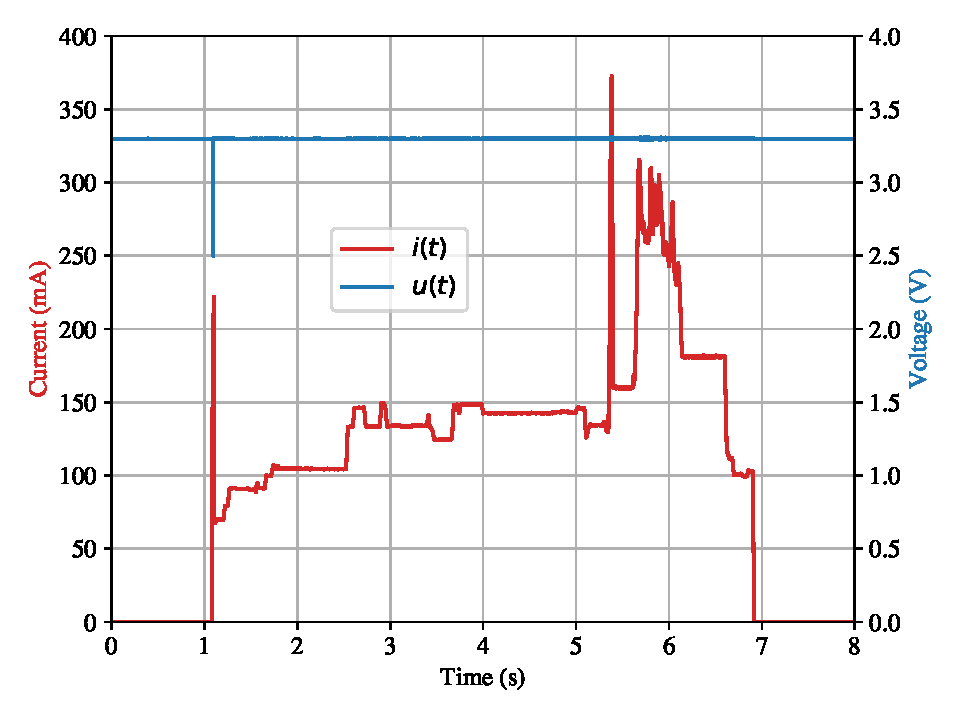
\includegraphics[width=0.9\textwidth]{5-results/energy/logger/ui.pdf}
	\caption{Current and Voltage during one write-cycle.\label{results:ui}}
\end{figure}
One write-cycle takes approximately 5.8 seconds.
In this interval, the STM32, nRF52480 and display driver are active.
Clearly visible is the inrush current peak.




\begin{figure}[ht]
	\centering
	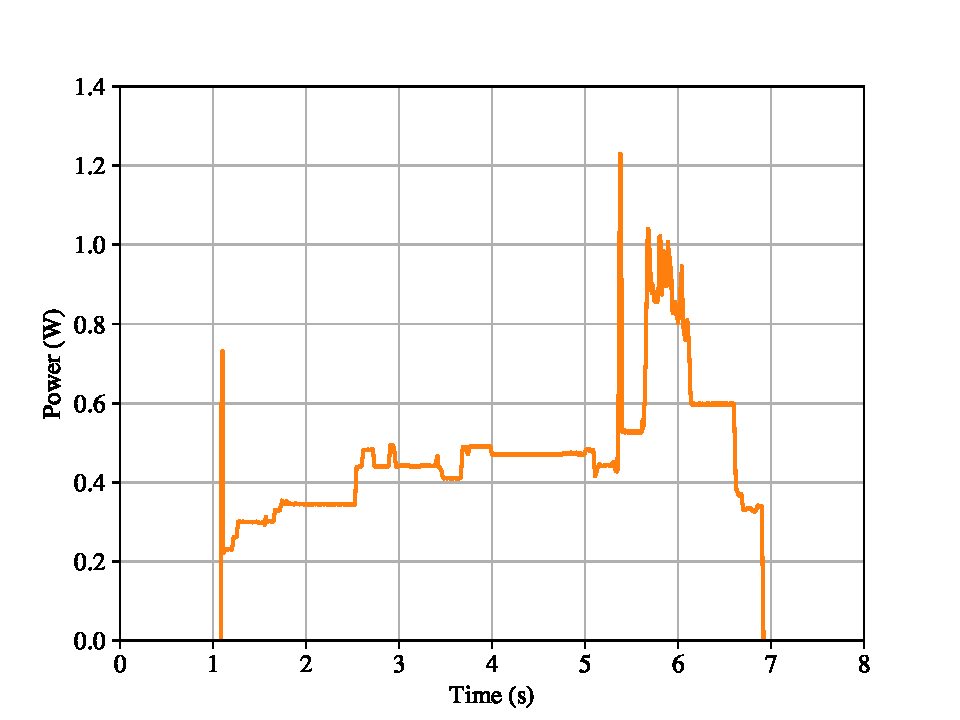
\includegraphics[width=0.9\textwidth]{5-results/energy/logger/p.pdf}
	\caption{Power consumption during one write cycle.\label{results:p}}
\end{figure}
\chapter{Summary}

%bibliography
\chapter*{Sources}
\addcontentsline{toc}{chapter}{Sources} 
\printbibliography[heading=none]

%Abbildungsverzeichnis
\addcontentsline{toc}{chapter}{List of figures} 
\listoffigures\thispagestyle{fancy}

%Tabellenverzeichnis
\addcontentsline{toc}{chapter}{List of tables} 
\listoftables\thispagestyle{fancy}

\addcontentsline{toc}{chapter}{Statement of Plagiarisms} 
\chapter*{Statement of Plagiarism}
%\textbf{Erkl�rung}\\
We declare that, apart from properly referenced quotations, this report is our
own work and contains no plagiarism; it has not been submitted previously
for any other assessed unit on this or other degree courses.
%Wir erkl�ren hiermit an Eides statt, dass ich die vorliegende Arbeit ohne Benutzung anderer als der angegebenen Hilfsmittel erstellt habe; die aus fremden Quellen direkt oder indirekt �bernommenen Gedanken sind als solche kenntlich gemacht. Die Arbeit wurde bisher in gleicher oder �hnlicher Form keiner anderen Pr�fungsbeh�rde vorgelegt und auch noch nicht ver�ffentlicht.\\
\vspace{0.8cm}\\

\begin{tabular}{l l}
    \textbf{Place} & \textbf{Date} \\
    Rapperswil  & \today
\end{tabular}
\vspace{0.8cm}

\textbf{Signatures}\\
\vspace{1.0cm}

Cedric Renda \hspace{3cm} Manuel Tischhauser

\clearpage



\appendix
\chapter{Requirements}

\newpage

\section{Assignment}
\begin{figure}[H]
	\centering
	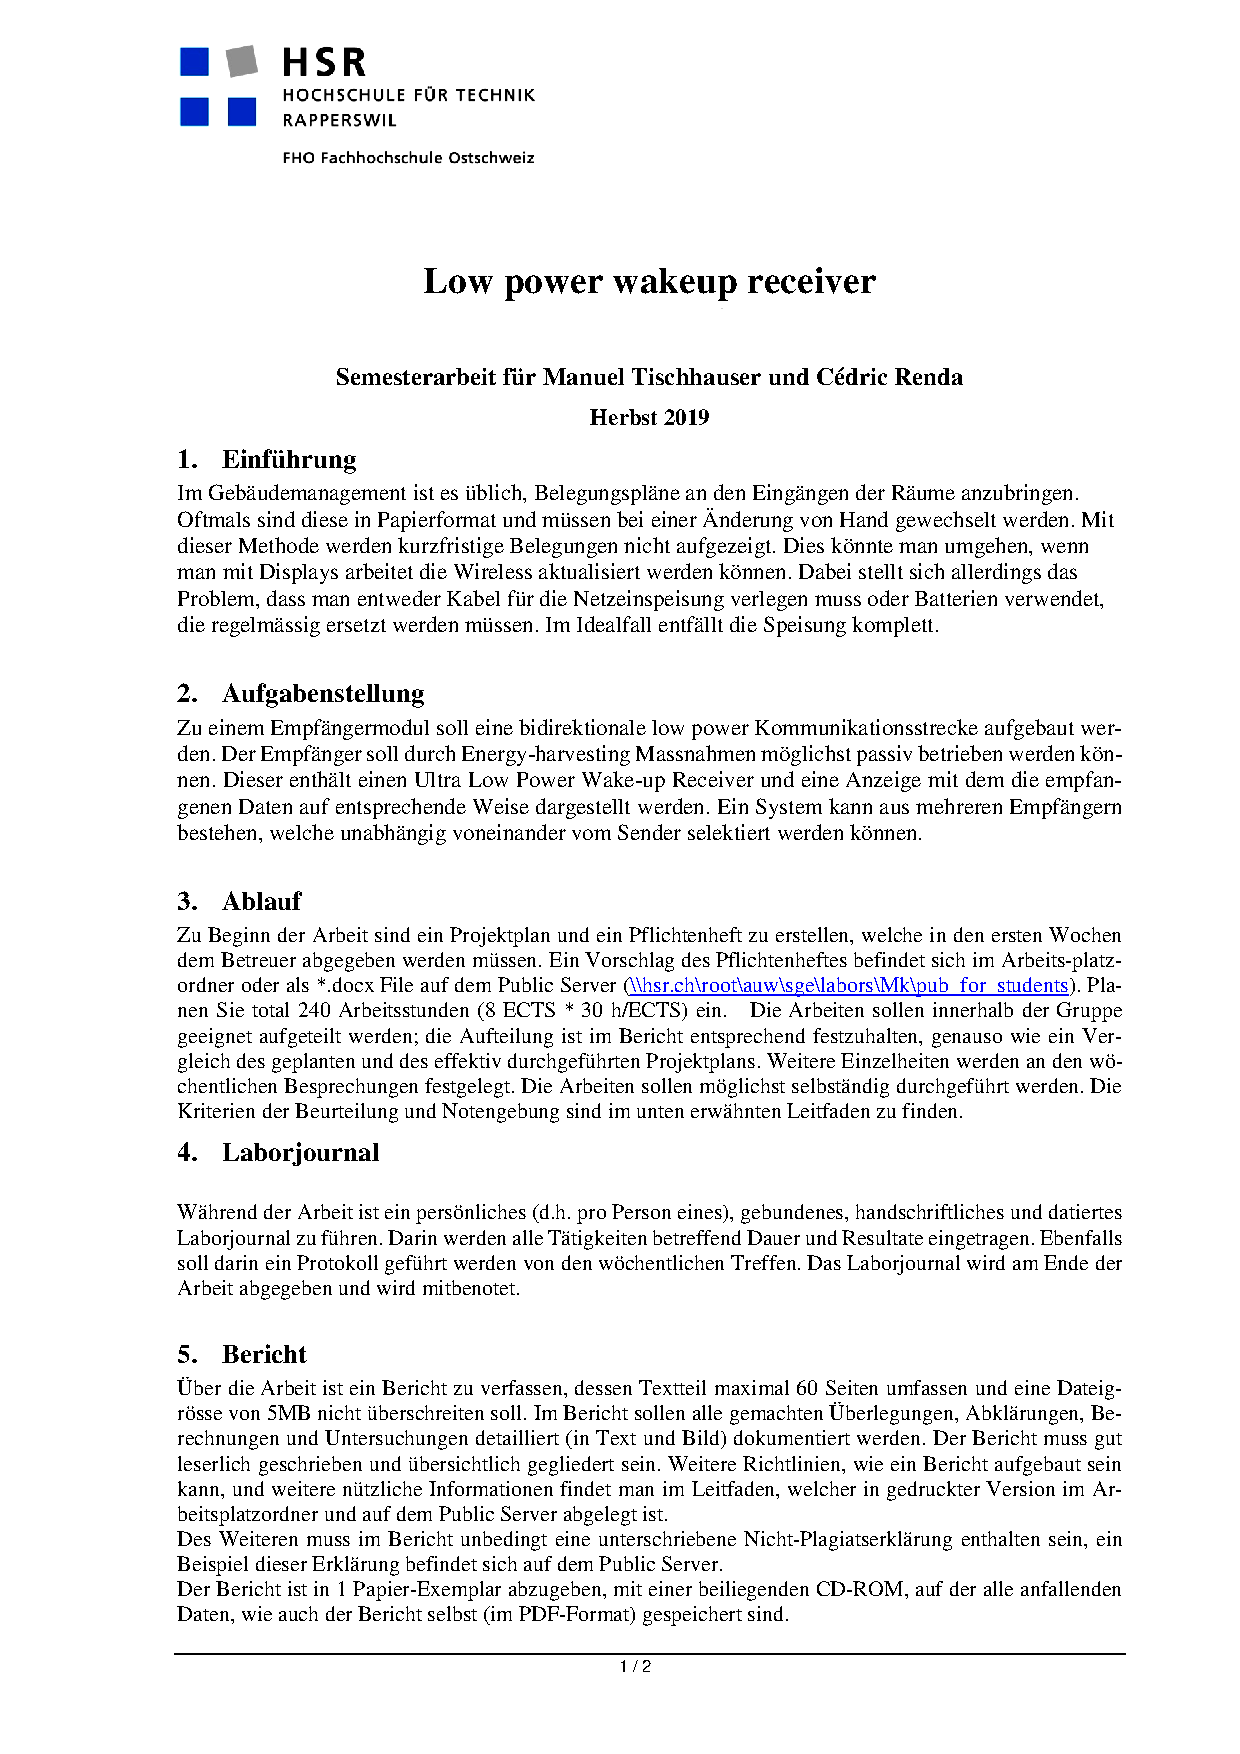
\includegraphics[trim= 0cm 0cm 0cm 0cm,page=1,width=16cm]{../Aufgabenstellung/LowPowerWakeupReiceiver.pdf}
\end{figure}
\begin{figure}[H]
	\centering
	\includegraphics[trim= 0cm 0cm 0cm 0cm,page=2,width=16cm]{../Aufgabenstellung/LowPowerWakeupReiceiver.pdf}
\end{figure}

\newpage
\section{Requirement Specification}
\begin{figure}[H]
	\centering
	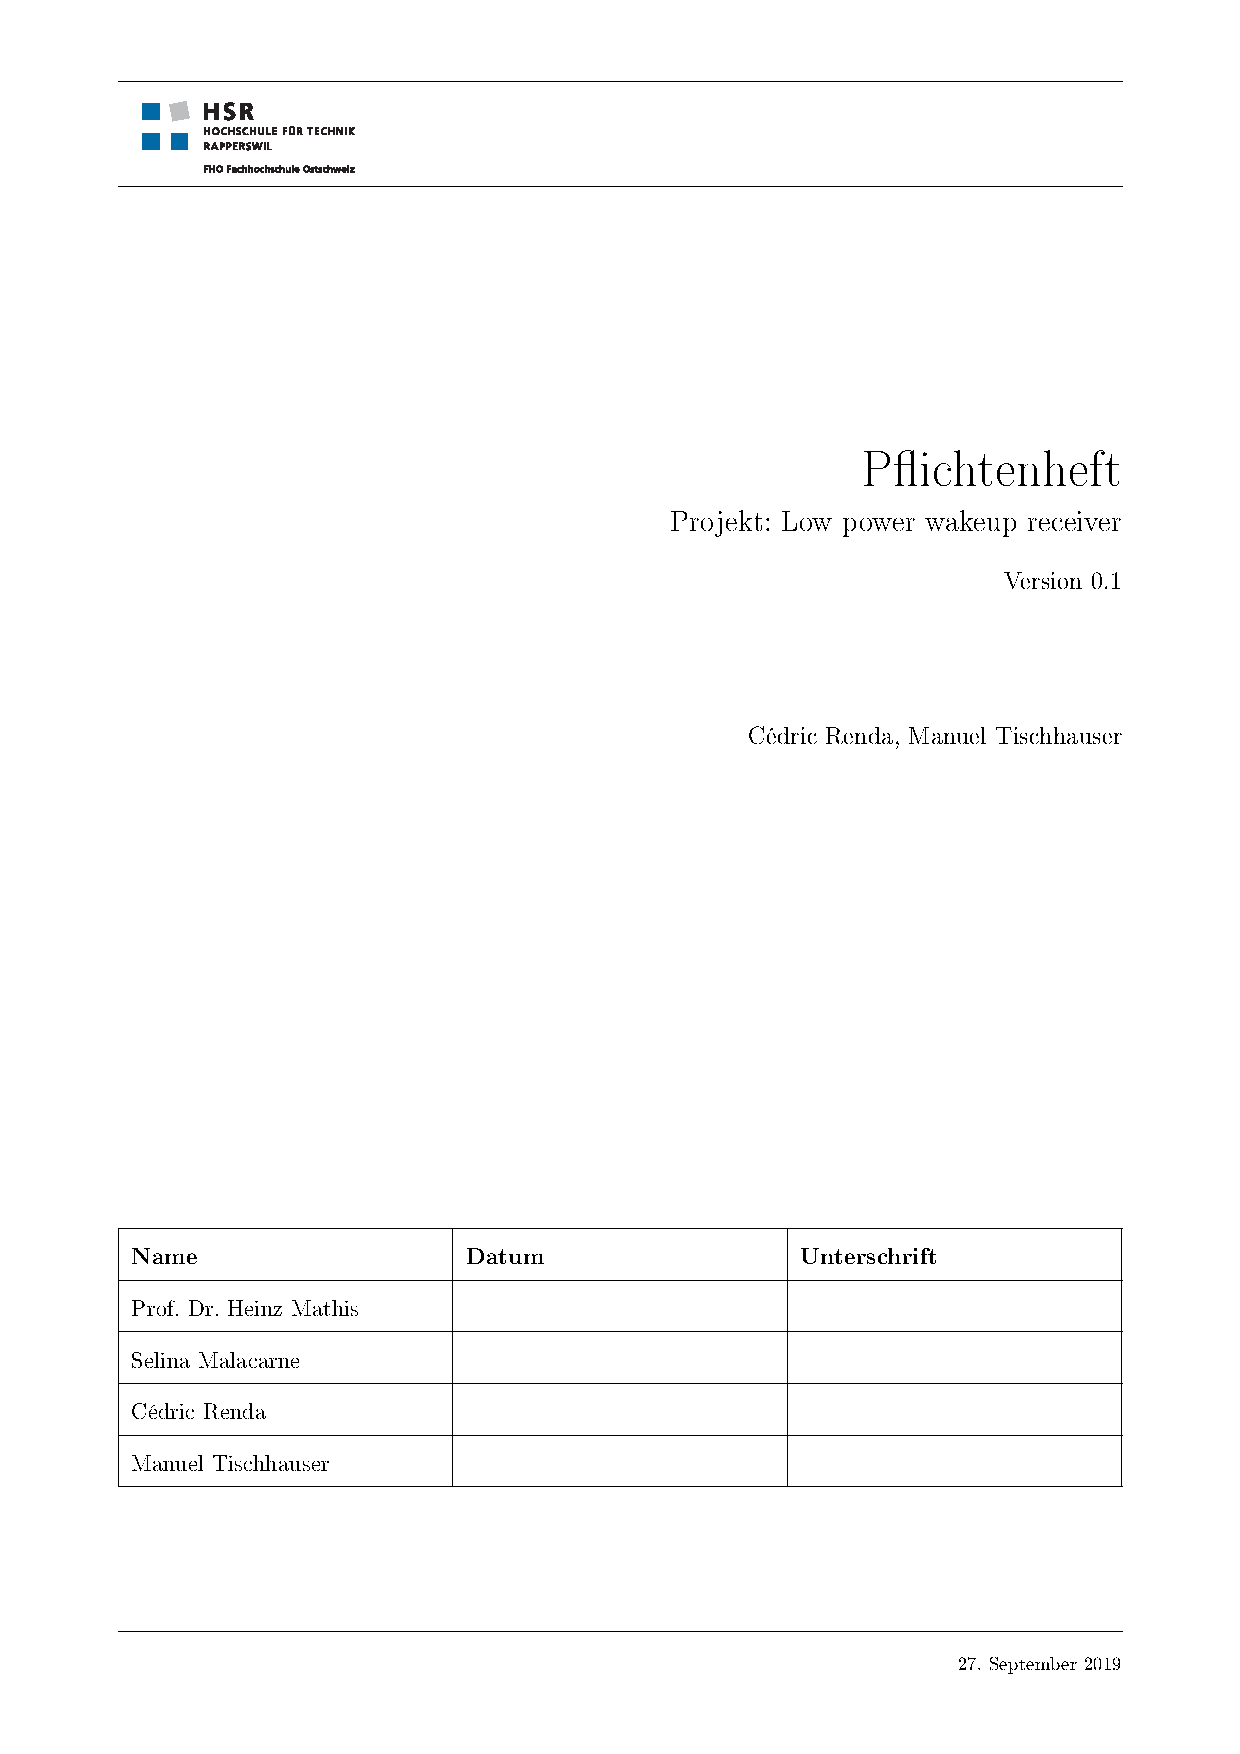
\includegraphics[trim= 0cm 0cm 0cm 0cm,page=1,width=16cm]{../Pflichtenheft/HSR_SRS_main.pdf}
\end{figure}
\begin{figure}[H]
	\centering
	\includegraphics[trim= 0cm 0cm 0cm 0cm,page=2,width=16cm]{../Pflichtenheft/HSR_SRS_main.pdf}
\end{figure}
\begin{figure}[H]
	\centering
	\includegraphics[trim= 0cm 0cm 0cm 0cm,page=3,width=16cm]{../Pflichtenheft/HSR_SRS_main.pdf}
\end{figure}
\begin{figure}[H]
	\centering
	\includegraphics[trim= 0cm 0cm 0cm 0cm,page=4,width=16cm]{../Pflichtenheft/HSR_SRS_main.pdf}
\end{figure}

\begin{landscape}
	\begin{figure}[H]
		\centering
		\includegraphics[trim= 0cm 0cm 0cm 0cm,page=5,width=22.56cm]{../Pflichtenheft/HSR_SRS_main.pdf}
	\end{figure}
\end{landscape}


\vfill
\pagebreak
\ifodd\value{page}\else\null\clearpage\fi
\lhead{Index}
\rhead{}
\addcontentsline{toc}{chapter}{\indexname}
\input main.ind
\end{document}
